\NeedsTeXFormat{LaTeX2e}[2005/12/01]
%%    2009/03/12 v1.0 GAUBM Vorlage für Aschlussarbeiten Physik
%% Template fuer Bachelor- und Masterarbeiten
%% an der Fakultaet fuer Physik (c) Thomas Pruschke der GA Universität
%% Verbesserungsvorschlaege bitte an pruschke@theorie.physik.uni-goettingen.de
%%
%% Benoetigte Pakete: datenumber
%%

%%%%%%%%%%%%%%%%%%%%%%%%%%%%%%%%%%%%%%%%%%%%%%%%%%%%%%%%%%%%%%%%%%%%%%
%%%%%%%%%% Bitte vor dem Veraendern diese Datei umbenennen! %%%%%%%%%%
%%%%%%%%%%%%%%%%%%%%%%%%%%%%%%%%%%%%%%%%%%%%%%%%%%%%%%%%%%%%%%%%%%%%%%

%% scrbook - Ersatz für LaTeX book Klasse aus dem KOMA Script
%% Moegliche Optionen: diejenigen der Klasse scrbook ausser titlepage

%% deutsche Arbeit:
\documentclass[bachelor,       %% Typ der Arbeit: bachelor oder master
               twoside,        %% zweiseitiges Layout
               BCOR10mm,       %% Bindekorrektur 10 mm
%               liststotoc,nomtotoc,bibtotoc, %% Aufnahme der div. Verzeichnisse
                                              %% ins Inhaltsverzeichnis
               english,ngerman, %% Alternativspr. Englisch, Dokumentspr. Deutsch
%               ngerman,english  %% Alternativspr. Deutsch, Dokumentspr. Englisch
%               final,          %% Endversion; draft fuer schnelles Kompilieren
               ]{GAUBM}

\usepackage{setspace}  %% Zur Setzung des Zeilenabstandes
\usepackage{babel}     %% Sprachen-Unterstuetzung
\usepackage{calc}      %% ermoeglicht Rechnen mit Laengen und Zaehlern
\usepackage[T1]{fontenc}       %% Unterstutzung von Umlauten etc.
%\usepackage[latin1]{inputenc}  %% 
%% in aktuellem Linux & MacOS X wird standardmaessig UTF8 kodiert!
\usepackage[utf8]{inputenc}    %% Wenn latin1 nicht geht ...

\usepackage{amsmath,amssymb} %% zusaetzliche Mathe-Symbole

\usepackage{lmodern} %% type1-taugliche CM-Schrift als Variante zur
                     %% "normalen" EC-Schrift
%% Paket fuer bibtex-Datenbanken
%\usepackage[comma,numbers,sort&compress]{natbib}
\usepackage{babelbib}
\selectbiblanguage{ngerman}
\bibliographystyle{apalike}

\newcommand{\tabheadfont}[1]{\textbf{#1}} %% Tabellenkopf in Fett
\usepackage{booktabs}                      %% Befehle fuer besseres Tabellenlayout
\usepackage{longtable}                     %% umbrechbare Tabellen
\usepackage{array}                         %% zusaetzliche Spaltenoptionen

%% umfangreiche Pakete fuer Symbole wie \micro, \ohm, \degree, \celsius etc.
\usepackage{textcomp,gensymb}

%\usepackage{SIunits} %% Korrektes Setzen von Einheiten
\usepackage{units}   %% Variante fuer Einheiten
\usepackage{xcolor}
%% Hyperlinks im Dokument; muss als eines der letzten Pakete geladen werden
\usepackage[pdfstartview=FitH,      % Oeffnen mit fit width
            breaklinks=true,        % Umbrueche in Links, nur bei pdflatex default
            bookmarksopen=true,     % aufgeklappte Bookmarks
            bookmarksnumbered=true  % Kapitelnummerierung in bookmarks
            ]{hyperref}

%% Weiter benoetigte Pakete: datenumber
%% Falls dieses Paket nicht in der Installation vorhanden ist,
%% kann es von der Seite mit diesem Template heruntergeladen werden
%% und in einem LaTeX bekanntem Verzeichnis installiert werden (notfalls
%% dem Verzeichnis mit der Arbeit).

% Mehrere Abbildungen nebeneinander
\usepackage{subfig}
\usepackage{adjustbox}

%Boxen,etc.
\usepackage{fancybox}
\usepackage{empheq}

% SI-Paket
\usepackage{siunitx}

%Matlab-Code
%\usepackage{listings}
\usepackage[framed,numbered]{matlab-prettifier}

\newcommand{\dif}{\ensuremath{\mathrm{d}}}

\begin{document}
%%
%%                   Ab hier muessen die Anpassungen geschehen
%%
%% Hier den eigenen Namen einsetzen
\ThesisAuthor{Felix}{Kurtz}
%% Hier den Geburtsort einsetzen
\PlaceOfBirth{Bad Nauheim}
%% Titel Arbeit. Das erste Argument ist der deutsche, das zweite der
%% englische Titel.
\ThesisTitle{Echtzeit-Spektroskopie der Multipuls-Dynamik in einem Ti:Sa-Femtosekunden-Oszillator}{Real-time spectroscopy of\\ multipulse dynamics in a \\Ti:Sapph femtosecond oscillator}
%% Erst- und Zweitgutacher/in
%% Ist der/die Betreuer/in nicht identisch mit dem/r Erstgutachter/in,
%% muss diese/r als optionales Argument angegeben werden.
\FirstReferee[Dr.\ Georg Herink]{Prof.\ Dr.\ Claus Ropers}
\Institute{4.Physikalischen Institut}
\SecondReferee{Prof.\ Dr.\ Stefan Mathias}
%% Beginn und Ende des Anfertigungszeitraumes
\ThesisBegin{1}{4}{2016}
\ThesisEnd{15}{7}{2016}
%% DO NOT TOUCH THESE LINES!!!!
\frontmatter
\maketitle
\cleardoublepage
%% Zusammenfassung. Falls nicht gewuenscht, bitte auskommentieren.
\begin{abstract}
  Hier werden auf einer halben Seite die Kernaussagen der Arbeit
  zusammengefasst.
%% Optional: Stichwoerter. Wenn nicht gewuenscht, koennen die beiden
%% folgenden Zeilen geloescht werden
  \bigskip\par
  \textbf{Stichwörter:} Physik, Bachelorarbeit
\end{abstract}
%% So laesst sich in die andere Sprache umschalten (Englisch bzw. Deutsch)
\begin{otherlanguage}{english}
\begin{abstract}
  Here the key results of the thesis can be presented in about
  half a page.
  \bigskip\par
  \textbf{Keywords:} Physics, Bachelor thesis
\end{abstract}
\end{otherlanguage}

%% Ende des Vorspanns
\cleardoublepage
%% Ab hier 1 1/2 facher Zeilenabstand (durch setspace-Paket)
\onehalfspacing
%% Erzeugt Inhaltsverzeichnis
\tableofcontents

%%% Hier kann man seine Bezeichnungsweisen erklaeren. Falls nicht
%%% benoetigt, bis einschliesslich \end{nomenclature} auskommentieren
%\begin{nomenclature}
%%% Fuer die Berechnung der Spaltenbreiten muss \usepackage{calc}
%%% geladen sein!
%\section*{Lateinische Buchstaben}
%\noindent
%\begin{longtable}[l]{p{0.2\textwidth}p{0.7\textwidth-6\tabcolsep}p{0.1\textwidth}}
%  \tabheadfont{Variable}&\tabheadfont{Bedeutung}&\tabheadfont{Einheit}\\\midrule\endhead
%  $A$ & Querschnittsfl"ache & $\unit{m^2}$\\
%  $c$ & Geschwindigkeit & $\unitfrac{m}{s}$
%\end{longtable}
%\section*{Griechische Buchstaben}
%\begin{longtable}[l]{p{0.2\textwidth}p{0.7\textwidth-6\tabcolsep}p{0.1\textwidth}}
%  \tabheadfont{Variable}&\tabheadfont{Bedeutung}&\tabheadfont{Einheit}\\\midrule\endhead
%  $\alpha$  & Winkel & $\unit{\degree}$; --\\
%  $\varrho$ & Dichte & $\unitfrac{kg}{m^3}$
%\end{longtable}
%\section*{Indizes}
%\begin{longtable}[l]{p{0.2\textwidth}p{0.8\textwidth-4\tabcolsep}}
%  \tabheadfont{Index}&\tabheadfont{Bedeutung}\\\midrule\endhead
%  m & Meridian\\
%  $r$ & Radial
%\end{longtable}
%\section*{Abk"urzungen}
%\begin{longtable}[l]{p{0.2\textwidth}p{0.8\textwidth-4\tabcolsep}}
%  \tabheadfont{Abk"urzung}&\tabheadfont{Bedeutung}\\\midrule\endhead
%  2D & zweidimensional\\
%  3D & dreidimensional\\
%  max & maximal
%\end{longtable}
%\end{nomenclature}
%% \listoftables und \listoffigures sollten nur bei genuegender Anzahl Tabellen
%% verwendet werden
%\listoffigures
%\listoftables

\mainmatter   %% Anfang Hauptteil

\chapter{Einleitung}
Femtosekundenlaser sind heutzutage aus der aktuellen Forschung nicht mehr wegzudenken.
Auch ihre Anwendungsgebiete werden vom industriellen Schneiden bis in den medizinischen Bereich immer vielfältiger.
Besonders Titan-Saphir:Laser sind der Standard im Labor, weil sie die kürzesten Pulse mit wenigen optischen Zyklen emittieren können.
Solch ein Laser ist ein nichtlineares System welches nicht nur auf Verstärkung und Verlusten basiert wie ein Dauerstrich-Laser (cw-Laser), der nur eine Wellenlänge emittiert.
Je kürzer der Puls, desto breiter muss dessen Spektrum sein.
In einem Femtosekundenpuls sind also viele Wellenlängen enthalten.
Diese haben im Lasermedium dispersionsbedingt unterschiedliche Ausbreitungsgeschwindigkeiten, was dazu führen würde, dass der Puls zerläuft.
Damit dies aber nicht geschieht und sich eine stabile Pulsform ausbildet, muss es zu  einem Gleichgewicht zwischen Dispersion und einem nichtlinearen Effekt kommen, welcher schnellere Frequenzen in langsamere wandelt -- und umgekehrt.
Die sich ausbildende Pulsformen werden \textbf{Solitonen} genannt.
Ein Titan:Saphir-Laser eignet sich also hervorragend, um deren Dynamik und Interaktionsmechanismen zu studieren.
Dazu müssen aber mehrerer Solitonen im Laser-Resonator umherlaufen.
Dies wird zwar in der Entwicklung von Ultrakurzpulslasern vermieden, da die dabei entstehenden Pulse länger sind als der mögliche Einzelpuls, durch eine höhere Pumpleistung sowie eine leichte Dejustage vom Optimalzustand lassen sich solche \textbf{Multipuls-Zustände} jedoch erzielen.
Davon berichtete zuerst \cite{lai_multiple_1997}.
Wie auch in den meisten späteren Beobachtungen wurde dort jedoch über viele Laserumläufe gemittelt.
Typische Ti:Sa-Oszillatoren haben nämlich eine Pulswiederholrate von etwa 80\,MHz.
Also werden auf einer Nanosekundenskala Pulse emittiert.
Der maximal mögliche Abstand zwischen zwei Pulsen, die im Laser umherlaufen, beträgt deshalb wenige Nanosekunden.
Solche Abstände lassen sich mit schnellen Photodioden auflösen, dies stellt experimentell also keine Hürde dar.
Interessant sind aber vor allem Abstände, die nur eine Größenordnung größer sind als die Pulsdauer, denn dann kommt es zu direkten Interaktionen zwischen den Pulsen.
Für Femtosekundenpulse liegt der spannende Abstandsbereich also unter einer Pikosekunde.
Dies ist zeitlich nicht mehr aufzulösen.
So muss der Pulsabstand entweder aus dem Spektrum bestimmt werden, denn dessen Fouriertransformation ist die Autokorrelation des Zeitsignals.
Typische Spektrometer besitzen jedoch einen CCD-Chip, auf den der Strahl zuvor spektral aufgespalten wird.
Ein solcher Chip 


In beiden Fällen

Dieses dynamische Verhalten konnte zuvor noch nicht in Echtzeit beobachtet werden.
Mit der hier genutzten Methode der \textit{dispersiven Fouriertransformation} sowie Hochgeschwindigkeitselektronik bestehend aus schnellen Photodetektoren und den schnellsten, kommerziell erhältlichen AD-Wandlern ist es nun möglich, das Spektrum jedes einzelnen Pulses bzw. Pulspaares aufzunehmen und in letzterem Fall daraus den Abstand sowie die Phase zwischen den beiden Pulsen zu bestimmen.
So lassen sich deutlich kleinere Pulsabstände auflösen als das im zeitlichen Signal jemals möglich wäre.
Dies eröffnet ganz neue Einblicke in die Welt der Laserdynamik.
Numerisch wurden schon vielfältigste Zustände modelliert, diese können nun erstmals im Experiment überprüft werden.

Mit dieser Echtzeit-Methode können außerdem erstmals auch transiente Dynamiken aufgelöst und somit die Prozesse im Laser besser verstanden werden.
Während \cite{herink_resolving_2016}

\chapter{Grundlagen}

\section{Ultrakurzpuls-Laser}
\subsection{Modelocking}
Damit ein Laser Femtosekundenpulse erzeugen kann, müssen viele Longitudinal-Moden im Resonator in Phase sein.
Dieses \emph{Modelocking} wird dadurch erreicht, dass hohe Intensitäten im Laser nichtlinear verstärkt werden.
Hier wird das durch den \textbf{Kerr-Effekt} erreicht, also den intensitätsabhängigen Teil des Brechungsindizes
\begin{align}
	n(I)=n_0+n_2\cdot I\,.
	\label{eq:kerr}
\end{align}
Da der Laserstrahl ein gaussförmiges Modenprofil hat, also exponentiell von der Strahlmitte in der Intensität abfällt, wirkt der Titan-Saphir-Kristall wie eine Linse.
Die Strahlmitte hat nämlich den längsten optischen Weg, während die äußeren Bereiche schneller durch den Kristall propagieren.

Höhere Intensitäten führen zu einer stärkeren Fokussierung des Strahls in das Laser-Medium.
Da dort auch der Pumpstrahl hinein fokussiert wird, ist in dessen Fokus die Besetzungsinversion höher und diese kann durch die stärkere Fokussierung effizienter abgebaut werden.
So wird dieser intensive Puls gegenüber dem cw-Signal bevorzugt und letzteres stirbt aus.
Dieses Verfahren wird \textbf{Soft aperture Modelocking} genannt, während beim \textit{Hard aperture Modelocking} einen Schlitz oder ähnliches benötigt wird.
Diese Apertur lässt den fokussierten, intensiven Strahl ohne Verlust passieren, während der cw-Anteil zum Teil adsorbiert wird und so hohe Verluste erfährt.

\subsection{Dissipative Solitonen}
Solitonen sind sehr stabile Pulse.
Sie beruhen auf einer Balance zwischen Dispersion, welches den Puls länger werden lässt, und einer Nichtlinearität, die den gegenteiligen Effekt hat.
So stellt sich eine sehr stabile Pulsform ein.
Dissipative Solitonen hingegen werden von einer weiteren Balance, nämlich zwischen Gewinnen und Verlusten, gehalten.
Sie können auch stabile Multipulsformationen bilden.


\section{Dispersive Fourier-Transformation}
Um das Spektrum jedes einzelnen Pulses vermessen zu können, wird eine lange Glasfaser genutzt, in die der Laserstrahl eingekoppelt wird.
Da ihr Brechungsindex frequenzabhängig ist, benötigen die unterschiedlichen Frequenzen des Femtosekunden-Pulses unterschiedlich lange, um durch die Glasfaser zu propagieren.
Die Länge der Glasfaser wird so angepasst, dass das ausgehende Signal etwas kürzer als die Puls-Wiederholrate des Lasers ist.
Dann kann das Spektrum am Ende der Faser mit einer schnellen Photodiode und einem schnellen Oszilloskop vermessen werden.
Dazu muss jedoch die Dispersion der Glasfaser bekannt sein, denn es kann nur der Zeitunterschied zwischen zwei Frequenzen gemessen werden, dieser muss aber noch den richtigen Frequenzen zugeordnet werden.
Falls der Laser stabil läuft und so Pulse mit immer dem gleichen Spektrum emittiert, kann dieses Spektrum auch mit einem herkömmlichen Gitter-Spektrometer gemessen werden.
Dabei wird der Strahl mit einem Gitter räumlich in seine spektralen Anteile zerlegt und diese dann mit einem CCD-Chip aufgenommen.
Da Letzter sehr langsam ist, wird somit automatisch über viele Pulse gemittelt und kann nur zur Kalibration genutzt werden.
Der Vorteil der obigen Methode ist nämliche die Beobachtung von sehr kurzen Prozessen, die sich nicht wiederholen.

Eine zeitliche Verschiebung im Signal nach der Faser könnte zwei Ursachen haben: eine zeitliche oder eine spektrale Verschiebung.
Deshalb wird mit einer zweiten Photodiode parallel noch das reine Zeitsignal aufgenommen, also der undispergierte Puls.

\subsection{Spektrale Interferenz und Doppelpulse}
Das Spektrum zweier gleichartiger Pulse, die einen bestimmten zeitlichen Abstand haben, weist eine Modulation auf, die invers zu diesem ist.
Dies lässt sich damit erklären, dass bestimmte Wellenlängen in Phase, andere aber außer Phase sind.
Mathematischer kann dies über folgende Eigenschaft begründet werden:
Die Fouriertransformation des Spektrums ist die Autokorrelation des zeitlichen Signals.

\section{Simulation}
Die Auswirkungen der oben beschriebenen optischen Elemente auf das elektrische Feld im Resonator können mathematisch beschrieben werden.
Dies resultiert in einer nichtlinearen partiellen Differentialgleichung vom Ginzburg-Landau-Typ.
Das hier beschriebene Modell wurde von \cite{kalashnikov_multipulse_2003} entwickelt, um Multipulse zu simulieren und damit Aussagen zu deren Stabilität machen zu können.
Es wird jedoch um die Berücksichtigung der Gaindynamik auf der Zeitskala des Simulationsfensters erweitert.


\subsection{Pulsformende Gleichung}
Zunächst komplexe Einhüllende $A(z,t)$ mit $z$ als und $t$ als 

\begin{align}
	\frac{\partial A(z,t)}{\partial z}=\left[\alpha-\rho-\frac{\gamma}{1+\sigma|A(z,t)|^2}+(t_f^2+iD)\frac{\partial^2}{\partial t^2}-i\beta |A(z,t)|^2\right]A(z,t)
\end{align}
Hierbei ist $\alpha$ die (zeitabhängige) lineare Verstärkung, $\rho$ der Verlust, $\gamma$ die Modulationstiefe des sättigbaren Absorbers, $\sigma$ die inverse Sättigungs-Intensität, $t_f$ die inverse Bandbreite der spektralen Verstärkung, $D$ die Dispersion und $\beta$ die Selbstphasenmodulation.

In der Simulation wird diese Gleichung numerisch per split-step-Verfahren gelöst.
Zeitliche Manipulationen werden im Realraum durchgeführt, während Dispersion und spektrale Verstärkung im Fourierraum angewendet werden.

\subsection{Gaindynamik}
Der lineare Gain $\alpha$, also die Besetzungsinversion, ist zeitabhängig.
Es gibt drei Terme, die diese ändern:
Das Pumpen, der Abbau durch stimulierte sowie durch spontane Emission, wobei die Änderung durch die beiden letzteren proportional zur aktuellen Besetzungsinversion sind, während die Änderung durch Pumpen proportional zur Differenz zwischen maximal erreichbarer Besetzungsversion $\alpha_\text{max}$ und dem aktuellen Wert ist.

%\begin{align*}
%	\frac{\dif \alpha(t)}{\dif t}_\text{pump}&\propto \alpha_\text{max}-\alpha(t)\\
%	\frac{\dif \alpha(t)}{\dif t}_\text{stimuliert}&\propto \alpha(t)\\
%\end{align*}
Man kann dies mit einem quasi 2-Level-System modellieren:
\begin{align}
	\frac{\dif \alpha(t)}{\dif t}=\frac{I_p\sigma_a}{h\nu_a}(\alpha_\text{max}-\alpha(t))-\frac{\sigma_g|A(z,t)|^2}{h\nu}\alpha(t)-\frac{\alpha(t)}{T_r}\,,
\end{align}
wobei $I_p$ die Pumpintensität, $\sigma_a$ der Absorptionsquerschnitt bei der Pumpfrequenz $\nu_a$ ist.
Weiter ist $\sigma_g$ der Verstärkungsquerschnitt bei der Laserfrequenz $\nu$ und $T_r$ die Lifetime des oberen Laserniveaus.

Davon ausgehend, dass das Pulspaar viel kürzer ist als die Resonatorlänge $T_\text{cav}$ und sich $\alpha$ während der Pulse vernachlässigbar ändert, kann die obige Gleichung mit $T_\text{cav}$ multipliziert und anschließend integriert werden:
\begin{align}
	\alpha(z)&=\alpha(z-1)\exp\left(-\frac{E}{E_s}-\frac{T_\text{cav}}{T_r}-P\right) \notag \\
	&+\frac{\alpha_\text{max}P}{\frac{E}{E_s}+\frac{T_\text{cav}}{T_r}+P}\left[1-\exp\left(-\frac{E}{E_s}-\frac{T_\text{cav}}{T_r}-P\right)\right]\,.
\end{align}
Hier ist $P=(I_p\sigma_a/h\nu_a)T_\text{cav}$ und $E_s=h\nu/\sigma_g$ sowie $E=\int_0^{T_\text{cav}}\dif t \,|A(z,t)|^2$.

Nun baut jedoch der erste Puls eines Pulspaars die Besetzungsinversion zumindest ein wenig ab, während Pumpen und spontane Emission auf dieser Zeitskala vernachlässigbar sind.
Die Berücksichtigung dieses Effekts stellt eine Erweiterung des Modells von \cite{kalashnikov_multipulse_2003} dar.
In erster Näherung ist
\begin{align}
	\alpha_2(z,t)&=-\frac{\alpha(z)}{E_s}\int_{t_1}^{t} \dif t'\, |A(z,t')|^2
\end{align}
Damit sich nun jedoch nicht das mittlere $\alpha$ ändert, muss von $\alpha_2$ noch der Mittelwert abgezogen werden bevor dieses $\alpha_\text{corr}$ zu $\alpha(z)$ addiert wird.
\begin{align}
	\alpha_\text{corr}(z,t)&=\alpha_2(z,t)-\int_{t_1}^{t_2} \dif t\, \alpha_2(z,t)\\
	\alpha(z,t)&=\alpha(z)+\alpha_\text{corr}(z,t)
\end{align}
Nun ändert sich der Gain auch wärend eines Roundtrips im Simulationsfenster.
Dies hat zur Folge, dass für zwei nicht-interagierende Pulse die Phasendifferenz linear durchläuft, denn der hintere ist immer ein wenig schwächer als der vordere.

\subsection{Experimentelle Parameter}

\chapter{Experimentelle Vorgehensweise}
\section{Laserquelle Femtolasers Rainbow}
Der zu untersuchende Laser ist ein Titan:Saphir-Laser (\textit{Rainbow} von \textit{FemtoLasers}).
Er erzeugt 7-fs-Pulse bei einer Puls-Wiederholrate von $78\,$MHz und einer Leistung von mehr als $250\,$mW.
Der Pumplaser ist ein frequenzverdoppelter, diodengepumpter Nd:YAG-Laser (\textit{Coherent Verdi V5}) mit bis zu 5\,W Leistung.
Der Ti:Sa-Kristall hat eine Länge von 2\,mm, in den der grüne Pumpstrahl mit einer 4\,cm-Linse fokussiert wird.
Um einen guten Kompromiss zwischen Stabilität und nichtlinearer Verstärkung im Pulsbetrieb zu erhalten \cite{stingl_sub-10-fs_1995}, ist der lange Arm etwa doppelt so lang wie der kurze.
Außerdem werden gechirpte Spiegel verwendet, um die Dispersion durch den Kristall auszugleichen.
Mit kleinen Prismen, den sogenannten Wedges, wird die Netto-Dispersion feingetunt.

Wenn der Laser angeschaltet wird, läuft er zunächst im cw-Betrieb.
Um nun in den Puls-Betrieb zu gelangen, muss der Endspiegel mit einem dafür vorgesehenen Knopf schnell bewegt werden.
Dadurch kommt es zu Intensitätsschwankungen, wovon eine stark genug sein muss, um genügend Verstärkung zu erfahren und damit das Modelocking zu starten.
\begin{figure}[!htb]
	\centering
	\includegraphics[width=0.8\textwidth]{figures/rainbow.png}
	\caption{Aufbau des \textit{Rainbow}s.}
	\label{fig:rainbow}
\end{figure}
\section{Detektions-Aufbau}
Der experimentelle Aufbau, um Echtzeit-Spektroskopie zu betreiben, ist sehr simpel.
Wie in Abb.\ref{fig:DFTSetup} zu sehen, wird der Laserstrahl zunächst mittels einer $\lambda/2$-Platte und einem Polarisator variabel abgeschwächt und senkrecht zur Tischebene polarisiert.
Danach passiert er einen optischen Isolator, welcher verhindert, dass Reflektionen an einer späteren Stelle bis in den Laser gelangen und dort zu unerwünschten Effekten bzw. Instabilitäten führen.
Als nächstes wird der Strahl mit einem Beamsplitter aufgeteilt.
Der transmittierte Anteil wird mit reflektiven ND-Filtern weiter abgeschwächt und mit einer Linse auf Photodiode Nr.2 fokussiert.
Diese misst also den undispergierten Puls.

Der vom Beamsplitter reflektierte Strahl wird in die Glasfaser eingekoppelt.
Um die Einkopplung zu ermöglichen/erleichtern läuft er zuvor noch über drei Spiegel, mit denen die Strahlposition und der Winkel eingestellt werden kann, mit dem der Strahl auf den Kollimator am Beginn der Glasfaser trifft.
Außerdem passiert er zuvor noch einen BK7-Kristall, in dem der Puls aufgrund der Dispersion etwas gestreckt wird, damit es am Anfang der Glasfaser nicht aufgrund zu hoher Intensitäten zu unerwünschten nichtlinearen Effekten kommt.
Am Ende der 400 Meter langen Glasfaser wird der Strahl mit einem Kollimator parallel ausgekoppelt und mit einer Linse auf Photodiode Nr.1 fokussiert, die also das dispergierte Signal/Spektrum misst.

Beide Photodioden sind an das Oszilloskop (Tektronix DP71604C) angeschlossen.
Dieses kann im 2-Kanal-Betrieb bis zu $4\,$ms mit einer Samplingrate von $25\,$GSa/s aufnehmen.
Dies entspricht mehr als 300\,000 Pulsen, denn die Pulswiederholrate des Lasers liegt bei $12.8\,$ns.


Um nun diese Technik der dispersiven Fouriertransformation richtig nutzen zu können, müssen die wichtigsten Bauteile charakterisiert werden: die Glasfaser sowie die beiden Photodioden.

\begin{figure}[!htb]
	\centering
	\def\svgwidth{\columnwidth}
	\input{DFTSetup2.pdf_tex}
	\caption{Setup Echtzeit-Spektroskopie: Laserstrahl wird mit einem Beamsplitter geteilt. Der eine Teil trifft direkt auf die Photodiode, der andere hingegen wird in einer dispersiven Faser auf Nanosekunden gestreckt und somit wird spektrale Information  in zeitliche  umgesetzt.}
	\label{fig:DFTSetup}
\end{figure}

\section{Kalibration der Dispersiven Fouriertransformation}
Zunächst muss die Dispersion in der Glasfaser gemessen werden, da mit dem Oszilloskop nur Zeitverzögerung gemessen werden kann und nicht direkt Frequenzen.
Dazu wird ein Etalon, hier ein Mikroskopie-Deckglas, genutzt, wenn der Laser stabil Einzelpulse liefert.
Aufgrund von Reflexionen an der Vorder- sowie Rückseite interferieren bestimmte Frequenzen konstruktiv, andere destruktiv.
Wie in \dots beschrieben, ergeben sich Frequenzabstände von
\begin{align*}
	\Delta \nu=\frac{c}{2Ln}\,,
\end{align*}
wobei $c$ die Lichtgeschwindigkeit, $n$ der Brechungsindex und $L$ die Länge des Materials ist.
Wird nun das Spektrum sowohl auf dem herkömmlichen Grating-Spektrometer  sowie mit dem Oszilloskop aufgenommen, kann anhand der Fringes im Spektrum den Frequenzen ein Delay nach der Glasfaser zugeordnet werden (Abb.\ref{fig:caliEtalon}).
Trotz des breiten Spektrums ergibt sich ein etwa linearer Zusammenhang
\begin{empheq}[box=\shadowbox]{align*}
  \frac{\Delta t}{\Delta \nu}=0.1082(8)\,\si{\nano\second\per\tera\hertz}
\end{empheq}
mit einer leichten Krümmung aufgrund Dispersion höherer Ordnung.
Dies bedeutet, dass pro Roundtrip, also 12.82\,ns, etwa 118\,THz aufgenommen werden und so eine zeitliche Auflösung von 8.44\,fs möglich ist.
Durch zeroPadding kann dies zwar noch erhöht werden,  die Daten werden dabei aber nur geglättet.

 \begin{figure}[!htb]
   \centering
   \subfloat[Spektrometer\label{fig:gratingEtalon}]
   {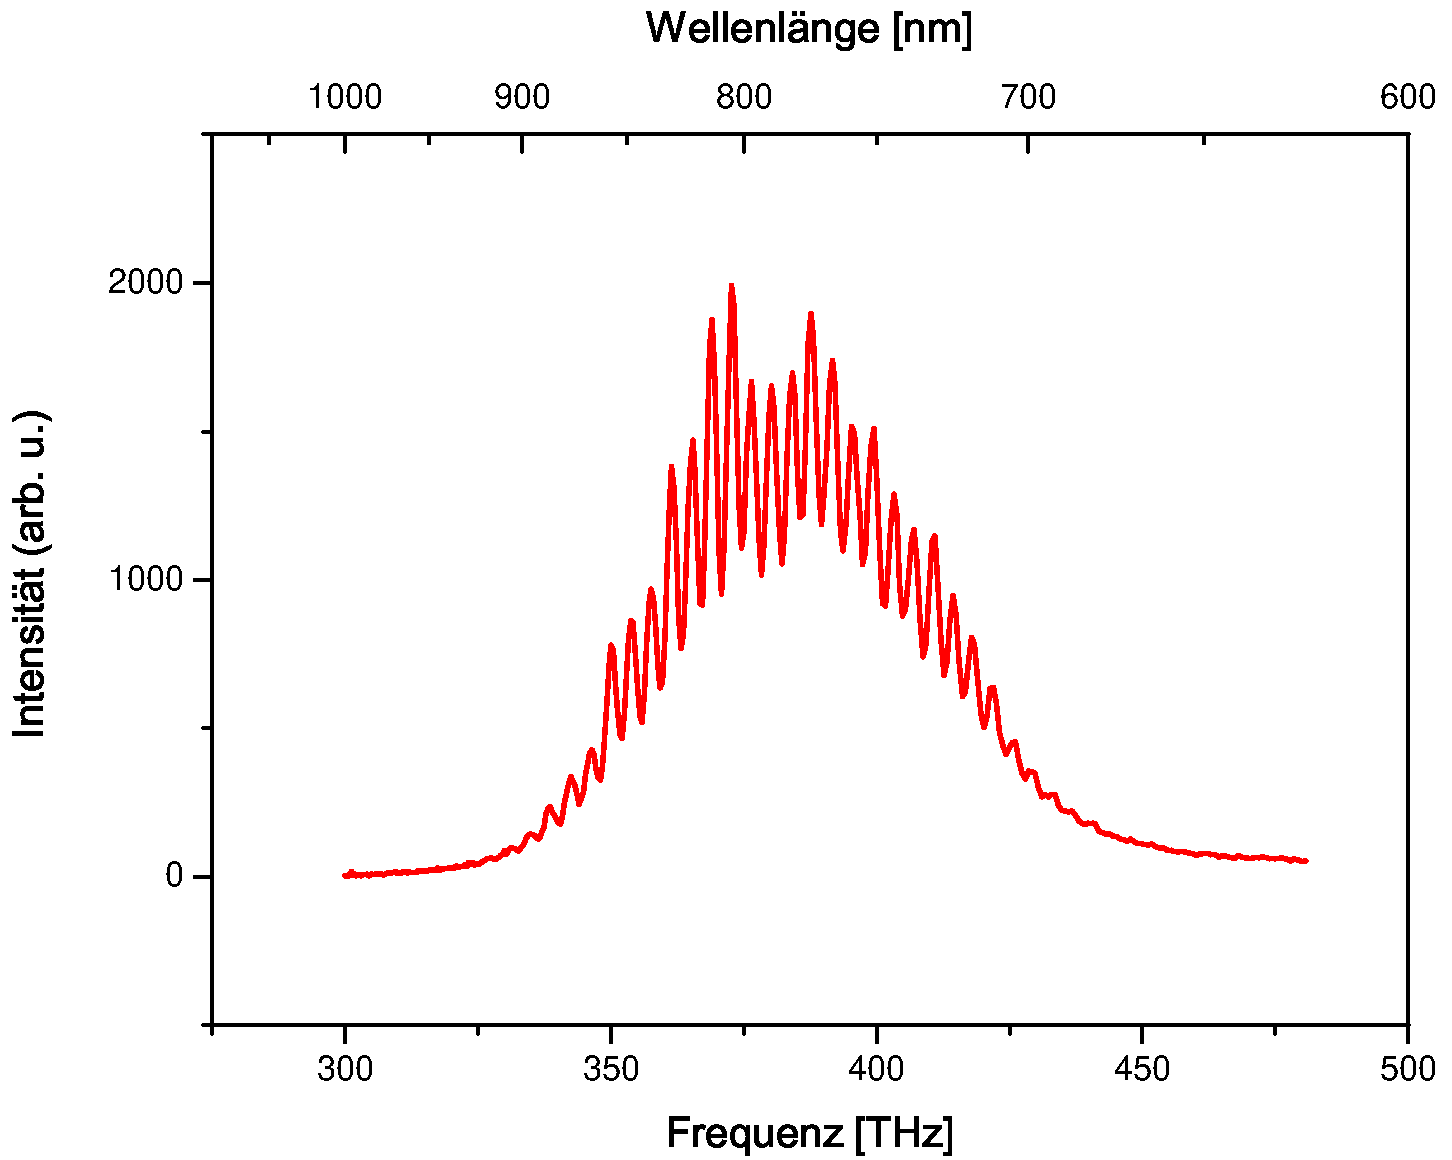
\includegraphics[width=0.49\textwidth]{figures/gratingEtalon}}
   \hfill
   \subfloat[Oszilloskop\label{fig:osziEtalon}]
   {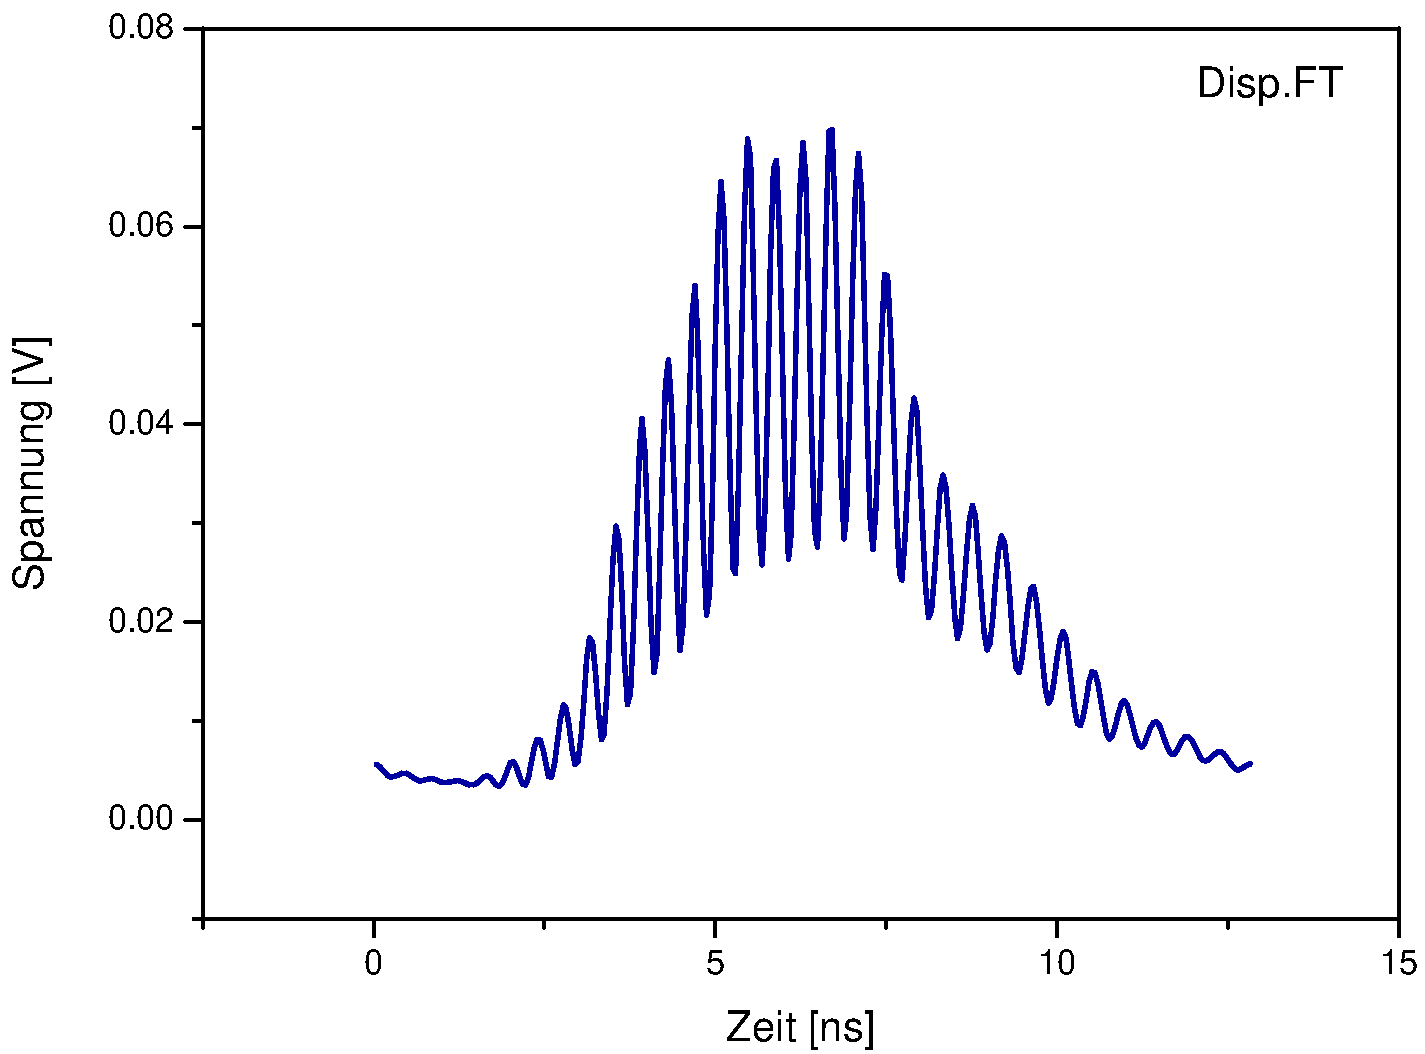
\includegraphics[width=0.49\textwidth]{figures/osziEtalon}}
   \hfill
   \subfloat[Kalibration\label{fig:calibration}]
   {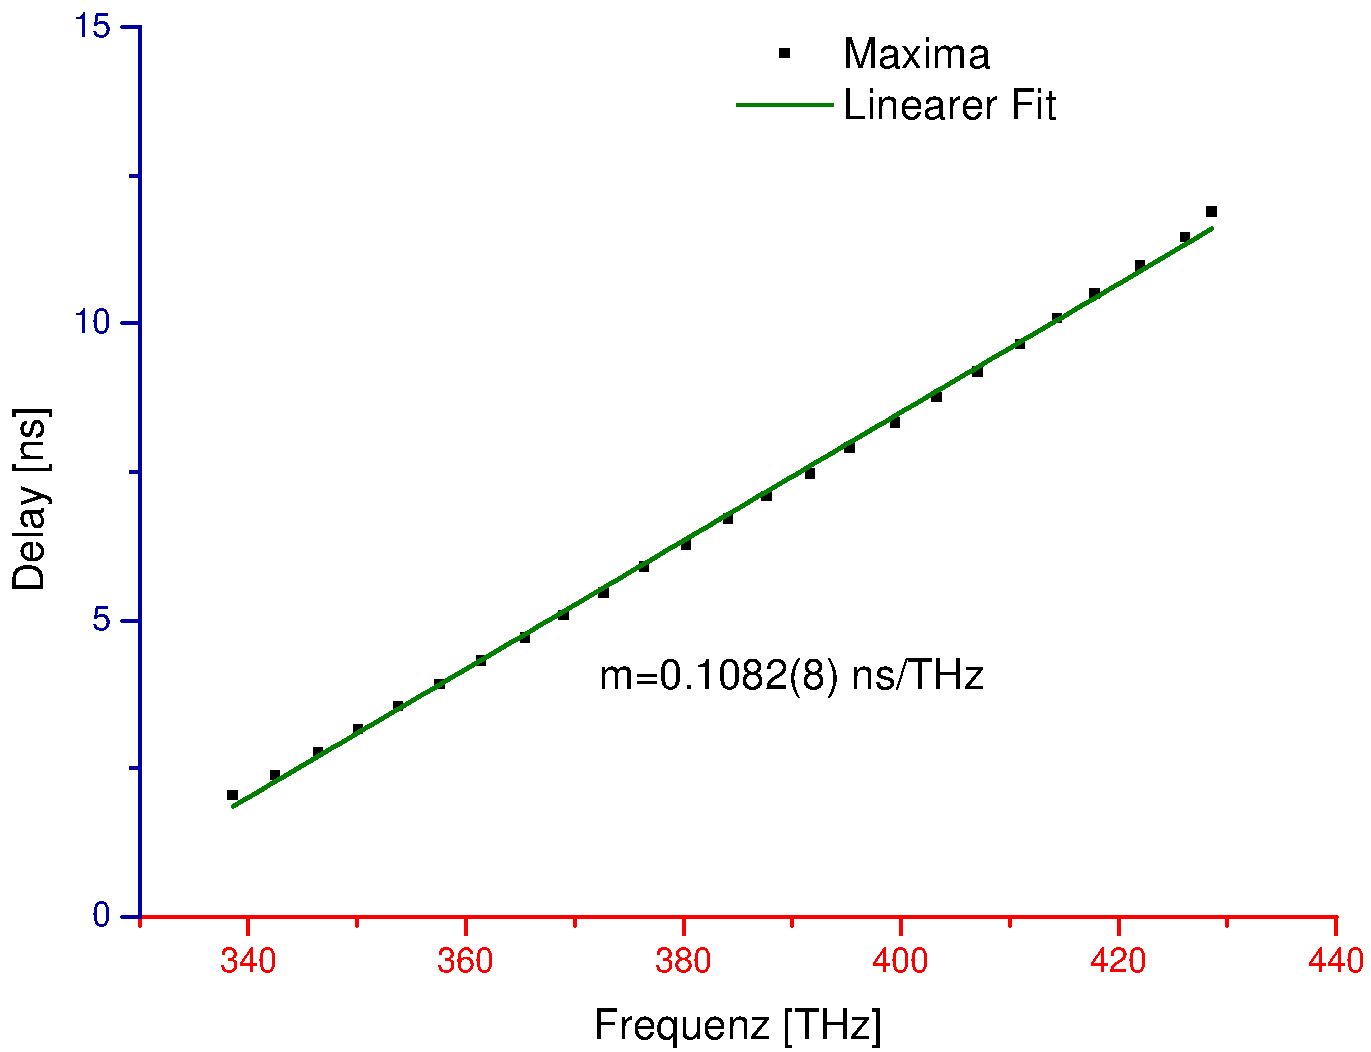
\includegraphics[width=0.6\textwidth]{figures/calibration}}
   \caption{Kalibration durch ein Etalon: Delay nach der Faser wird zu Frequenzen zugeordnet.}
   \label{fig:caliEtalon}
 \end{figure}

\section{Charakterisierung der Photodioden}
Als nächstes muss noch die Photodiode (Alphalas UPD-40-UVIR-P) charakterisiert werden.
In Tabelle \ref{tab:PD} finden sich die wichtigsten Herstellerangaben zu diesem ultraschnellen Photodetektor.
Diese sollen überprüft bzw. auf die experimentelle Situation hin getestet werden.
Nun werden 2 Photodioden für das Experiment eingesetzt.
Um diese zu unterscheiden, bekam die eine ein Label, im Folgenden mit \texttt{CRC-Label} gekennzeichnet.
Die andere wird im Folgenden mit \texttt{noLabel} bezeichnet.

Zunächst wird getestet, in welchem Leistungsbereich die Photodioden linear reagieren, damit bei zukünftigen Messungen dieser Bereich nicht überschritten wird.
Dies muss für die beiden Messmodi mit undispergiertem sowie dispergiertem Signal geschehen.
Außerdem muss noch die Bandbreite der Photodiode abhängig von der eingestrahlten Leistung bestimmt werden, denn für die Beobachtung von relativ weit entfernten Pulsen (bis zu 1\,ps) ist es wichtig, dass die Photodiode schnell reagiert.
Diese Pulse sind zu nah, um sie im zeitlichen Signal getrennt zu sehen.
So können sie gerade noch als spektrale Interferenz wahrgenommen werden.

Um die Leistungsabhängigkeiten zu messen, wird der Laserstrahl mit der $\lambda/2$-Platte variabel abgeschwächt, mit einem Powermeter direkt vor der entsprechenden Photodiode wird dies kontrolliert.

\begin{table}[!htb]
	\centering
	\begin{tabular}{|c|c|}
		\hline
		PD. Spezifikation & Wert \\		
		\hline
		Risetime & < 40\,ps \\
		Bandbreite & >8.5\,GHz \\
		Spektraler Bereich & 350-1700\,nm \\
		Sensitivität @ 800\,nm & 0.12\,A/W\\
		\hline	
	\end{tabular}
	\caption{Herstellerangaben zur Photodiode Alphalas UPD-40-UVIV.}
	\label{tab:PD}
\end{table}

\subsection{Antwort auf undispergiertes Signal}
In Abbildung \ref{fig:PDundisp} wird in Abhängigkeit der eingestrahlten Leistung die Photodiodenantwort auf das undispergierte Signal dargestellt, also auf einen kurzen Puls, dessen Dauer viel geringer als die Risetime der Photodiode ist.
Um dies zu messen, wird der Laserstrahl so auf die Photodiode gerichtet, dass er auf den sensitivsten Bereich trifft.
Dazu wird die Linse vor der Photodiode richtig positioniert.
Erkennbar ist, dass die Peakamplitude bis ca. 2\,mW linear ansteigt und in dieser Region die Pulsbreite (FWHM) etwas über 100\,ps liegt.
Dies ist verträglich mit der angegebenen Risetime von 40\,ps.
Außerdem ist je nach Justage ein Ringing nach dem Puls zu beobachten.

\begin{figure}[!htb]
	\centering
	\subfloat[Antwortverhalten der beiden Photodioden: Bei steigender Leistung sättigt die Peakspannung und die Photodioden-Antwort wird länger.\label{fig:PDfwhmMaxI}]
   {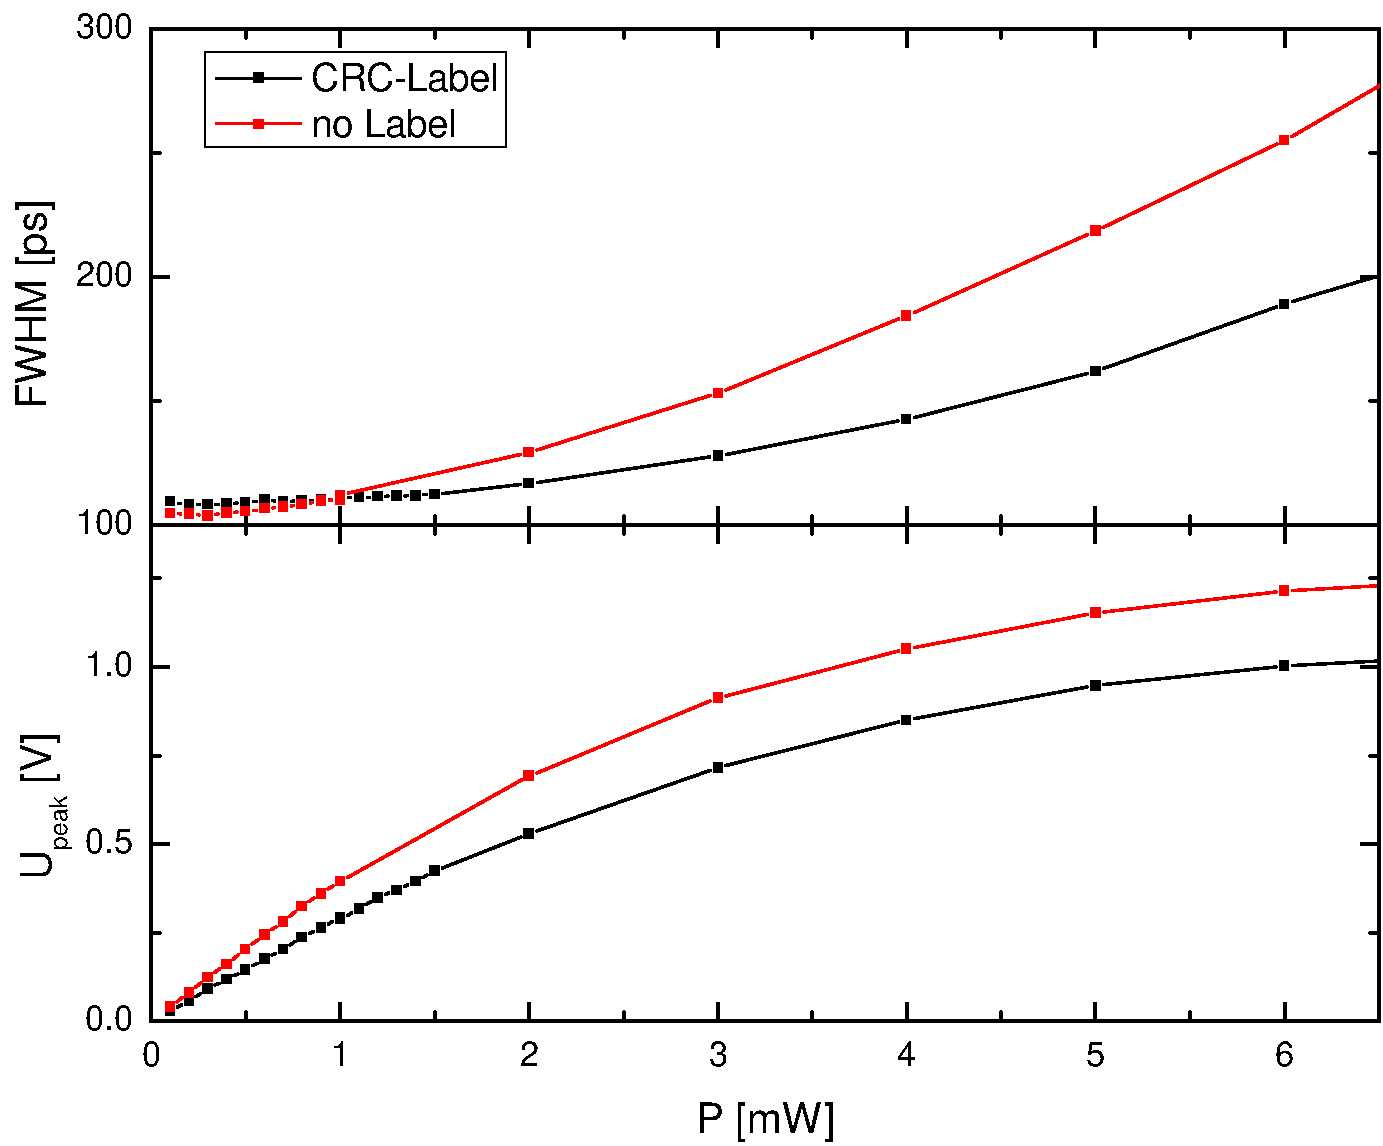
\includegraphics[width=0.49\textwidth]{figures/PDfwhmMaxI}}
   \hfill
   \subfloat[Vergleich der beiden Dioden bei 2\,mW: Unterschied kann auch auf Einstrahlung zurückzuführen sein. \label{fig:PD2mW}]
   {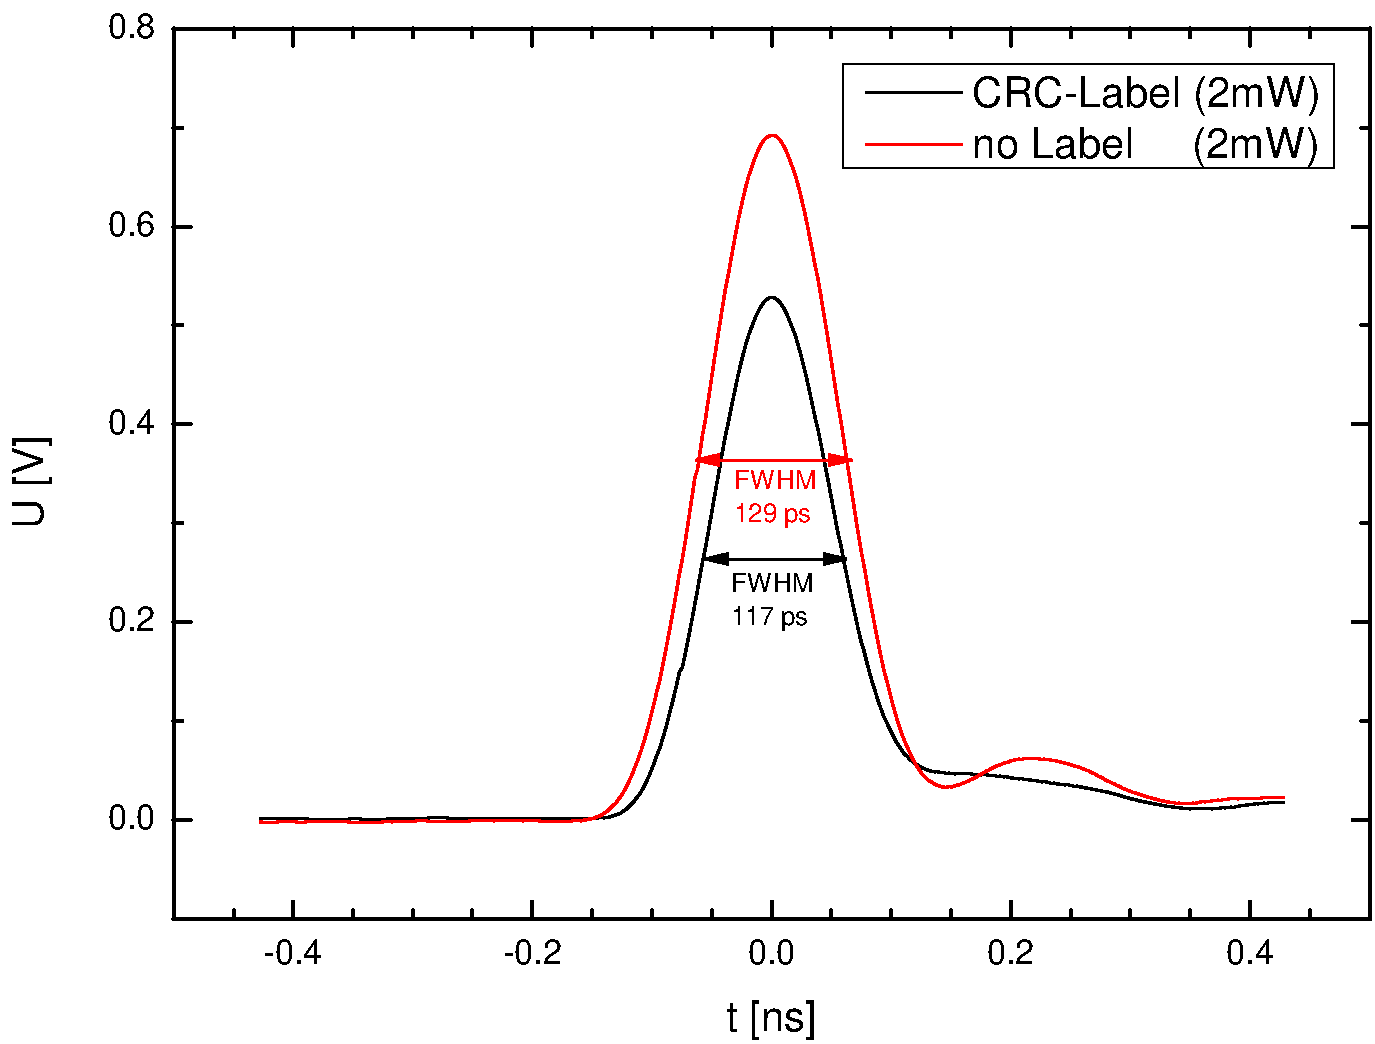
\includegraphics[width=0.49\textwidth]{figures/PD2mW}}
	\caption{Undispergiert}
	\label{fig:PDundisp}
\end{figure}


\subsection{Antwort auf dispergiertes Signal}
Bis ca. 10\,mW wächst das Signal linear an.
Danach wird die Photodiode übersteuert, sodass nicht genug Ladungsträger zwischen zwei Pulsen nachfließen können.
Die Pulsform ändert sich komplett und das Signal ist nicht mehr nützlich.
Im linearen Bereich kann allerdings die Sensitivität der Photodiode bestimmt werden, also welcher Strom bei einer bestimmten eingestrahlten Leistung von der Photodiode produziert wird.
Um den geflossenen Strom zu erhalten, wird die am Oszilloskop anliegende Spannung durch den benutzen Widerstand von $50\,\si\ohm$ geteilt.
Außerdem muss der Strom noch über einen Roundtrip gemittelt werden, denn die eingestrahlte Leistung ist auch nur als Mittlung messbar.
In Abb. \ref{fig:PDdispMeanA} wird dies für beide Photodioden bestimmt und beide liefern sehr ähnliche Sensitivitäten: 0.1154(8)\,A/W für  \texttt{CRC-Label} und  0.1120(5) für \texttt{noLabel}.
Der kleine Unterschied kann auch durch die \dots bedingt sein.
Insgesamt sind beide Werte aber im guten Einklang mit der aus dem Datenblatt entnommenen Sensitvitätskurve in Abb.\ref{fig:PDsensDB}

\begin{figure}[!htb]
	\centering
	\subfloat[\label{fig:PDdispMeanA}]
   {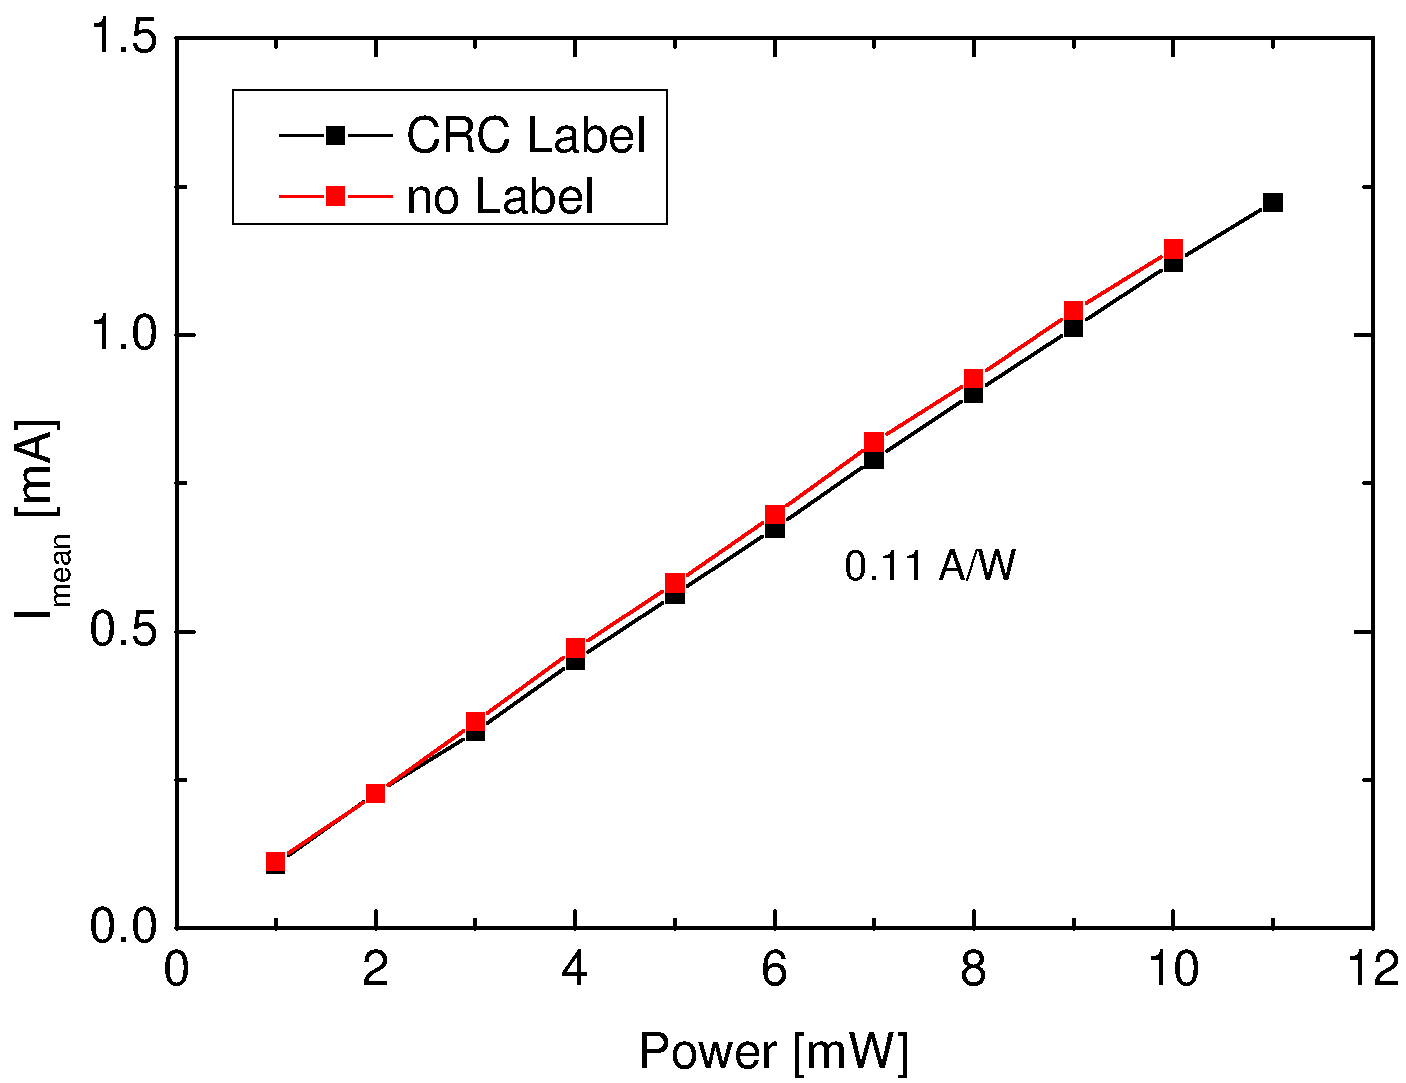
\includegraphics[width=0.44\textwidth]{figures/PDdispMeanA}}
   \hfill
   \subfloat[Sensitivität aus dem Datenblatt\label{fig:PDsensDB}]
   {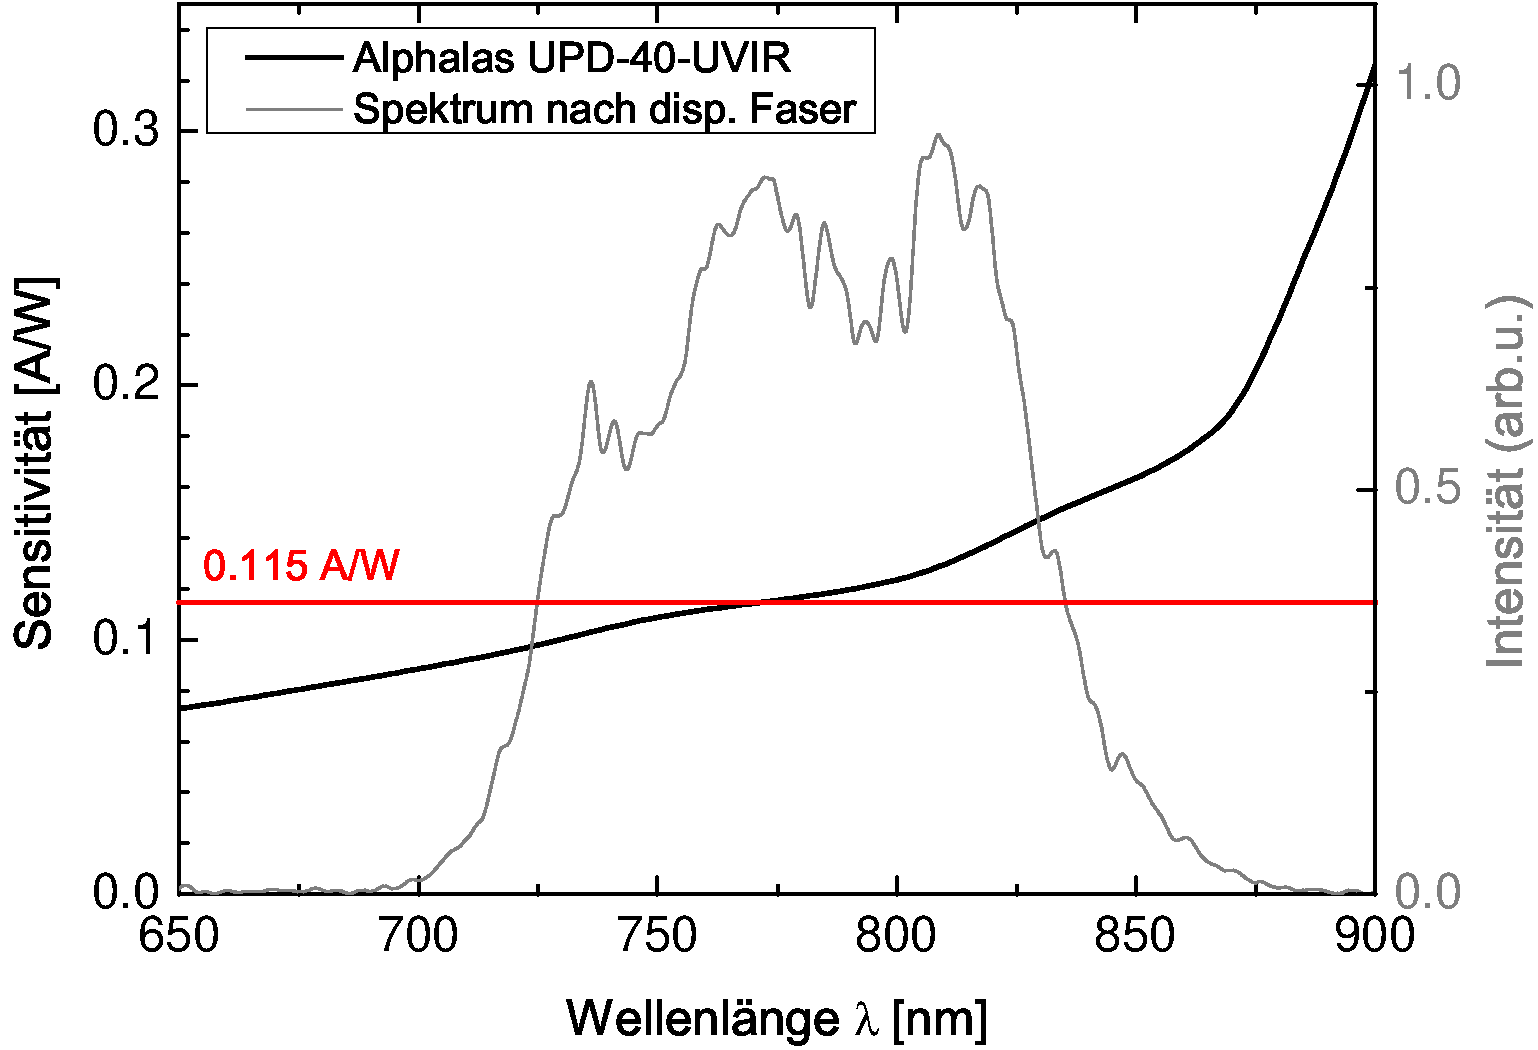
\includegraphics[width=0.49\textwidth]{figures/PDsensitivty}}
	\caption{Sensitivität der Photodioden}
	\label{fig:PDsens}
\end{figure}


\subsection{Bandbreite}
Das Spektrum sollte voll durchmoduliert sein, wenn beide Pulse gleich stark sind.
Die Photodiode wird jedoch ab einer bestimmten Modulationfrequenz, also einem bestimmten Abstand der Doppelpulse nicht so schnell reagieren können, dass das Signal komplett auf 0 heruntergeht.
Dadurch wird der Intensitätsunterschied der beiden Pulse überschätzt.
Um dies zu untersuchen, wird ein Michelson-Interferometer in den Strahlengang eingebaut.
Mit diesem kann durch Variation der einen Armlänge für unterschiedliche Abstände zwischen den beiden Pulsen aus beiden Armen gesorgt werden.
Diese Abstände finden sich in der Modulation des Spektrums wieder.

\chapter{Ergebnisse}
In diesem Kapitel wird zunächst erläutert, wie der Resonator justiert sein muss, um Multipulse erzeugen zu können.
Danach wird erklärt, wie die Messdaten bearbeitet werden, damit man aus ihnen Pulsabstände bestimmen kann.
Mit diesem Vorwissen werden dann die beobachteten Multipulse dargestellt.
Dabei wird sich hier auf Multipulse mit geringen Pulsabständen ($< 1\,$ps) beschränkt.
Wie schon von \cite{lai_multiple_1997} beschrieben, gibt es aber auch Multipulszustände, bei denen sich je zwei Pulse genau im Kristall treffen und so auch den Kerr-Effekt des jeweils anderen spüren.
Im Abschnitt \ref{sec:cpml} wird auf diesen Effekt genauer eingegangen.

\section{Kartierung des Resonators}
Für das Einstellen von Multipulsen ist die Kenntnis der wichtigsten Resonatorparameter nötig.
Dazu gehört die Kristallposition und der Abstand zwischen den beiden fokussierenden Spiegeln.
Da die Abstände nur sehr gering geändert werden ($\sim 100\,\si{\micro\meter}$), ist die Messung dieser etwas ungenau.
Gemessen wird nämlich von außen durch Anhalten eines digitalen Messschiebers, dessen Genauigkeit  bei ca. $10\,\si{\micro\meter}$ liegt.

In Abbildung \ref{fig:map} wird der Abstand der fokussierenden Spiegel bei verschiedenen Kristallpositionen variiert.
In Abhängigkeit dessen wird mit einem Powermeter direkt am Laserausgang die cw-Leistung und -- wenn möglich -- auch die gemodelockte Leistung gemessen.
Zu erkennen ist, dass die cw-Leistung geringer wird, wenn der Abstand zwischen den beiden Spiegeln verringert wird.
Dies ist auch der typische Weg, den Laser zu justieren.
Zuerst wird die cw-Leistung durch Justage der Resonator-Endspiegel maximiert.
Danach wird der Abstand der beiden Fokussierspiegel verringert, während der Endspiegel bewegt wird, um Fluktuationen zu erzeugen, die bei geeigneter Stellung modelocken.
Des weiteren ist die Ausgangsleistung im gemodelockten Betrieb größer als die cw-Leistung und nahezu unabhängig von der Stabilitätsposition.


\begin{figure}[!htb]
	\centering
	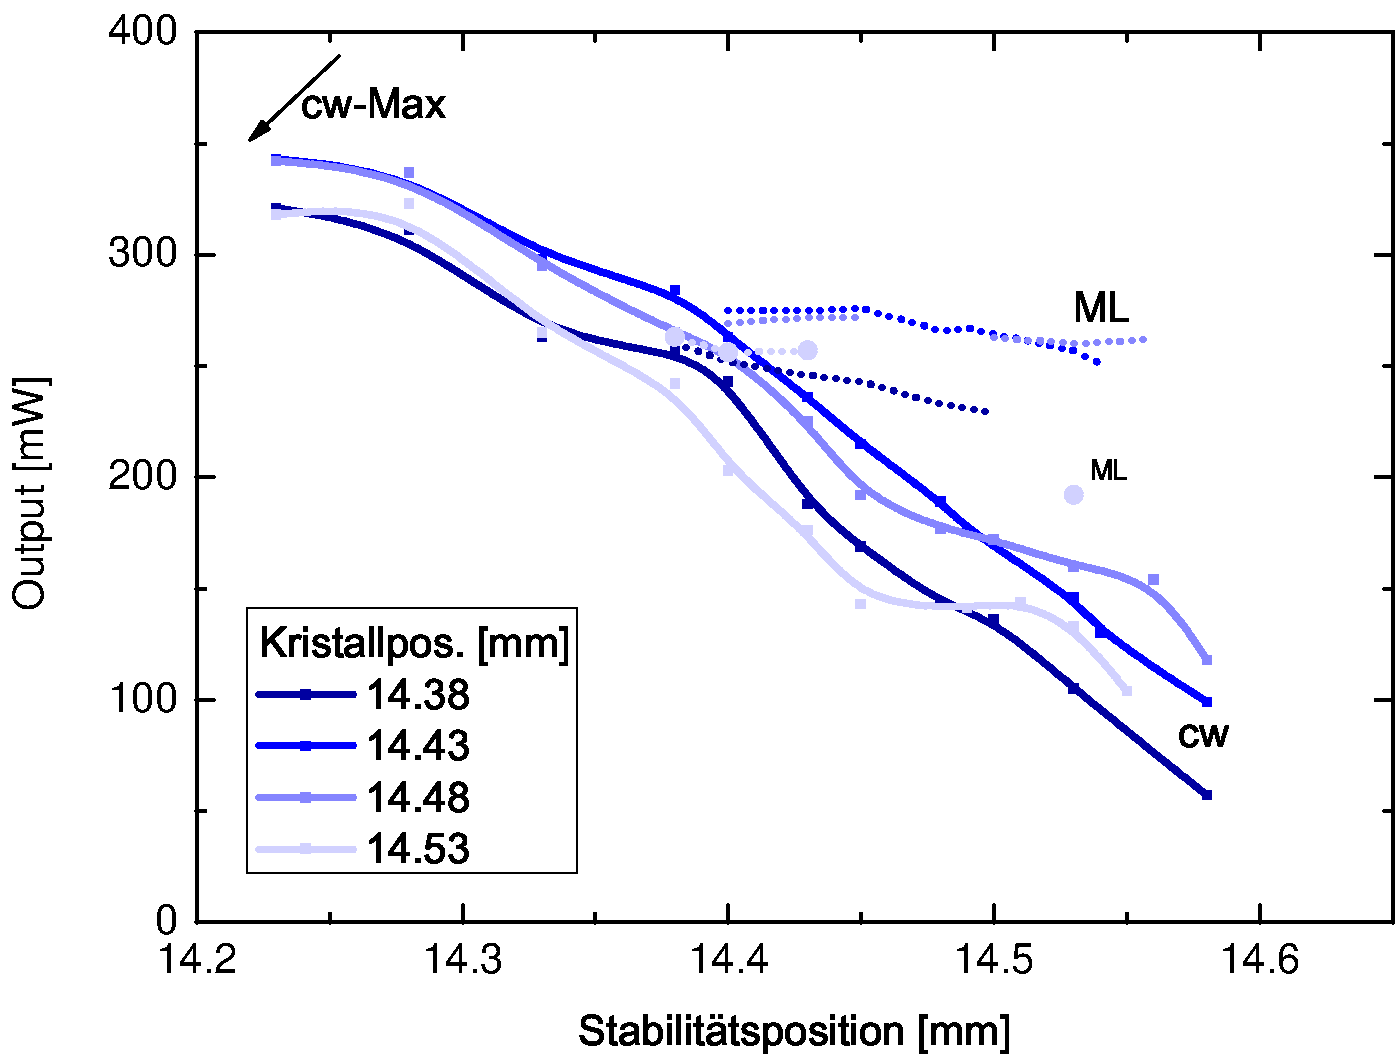
\includegraphics[width=0.7\textwidth]{figures/map.pdf}
	\caption{Abhängigkeit der Leistung (cw \& gemodelockt) von der Position des fokussierenden Spiegels (Stabilität) bei verschiedenen Kristallpositionen.
	Die Positionen werden von außen gemessen, dh. dass größere Werte einer Verringerung des Abstandes zum festen Fokussierspiegel entsprechen.}
	\label{fig:map}
\end{figure}

\begin{figure}[!htb]
	\centering
	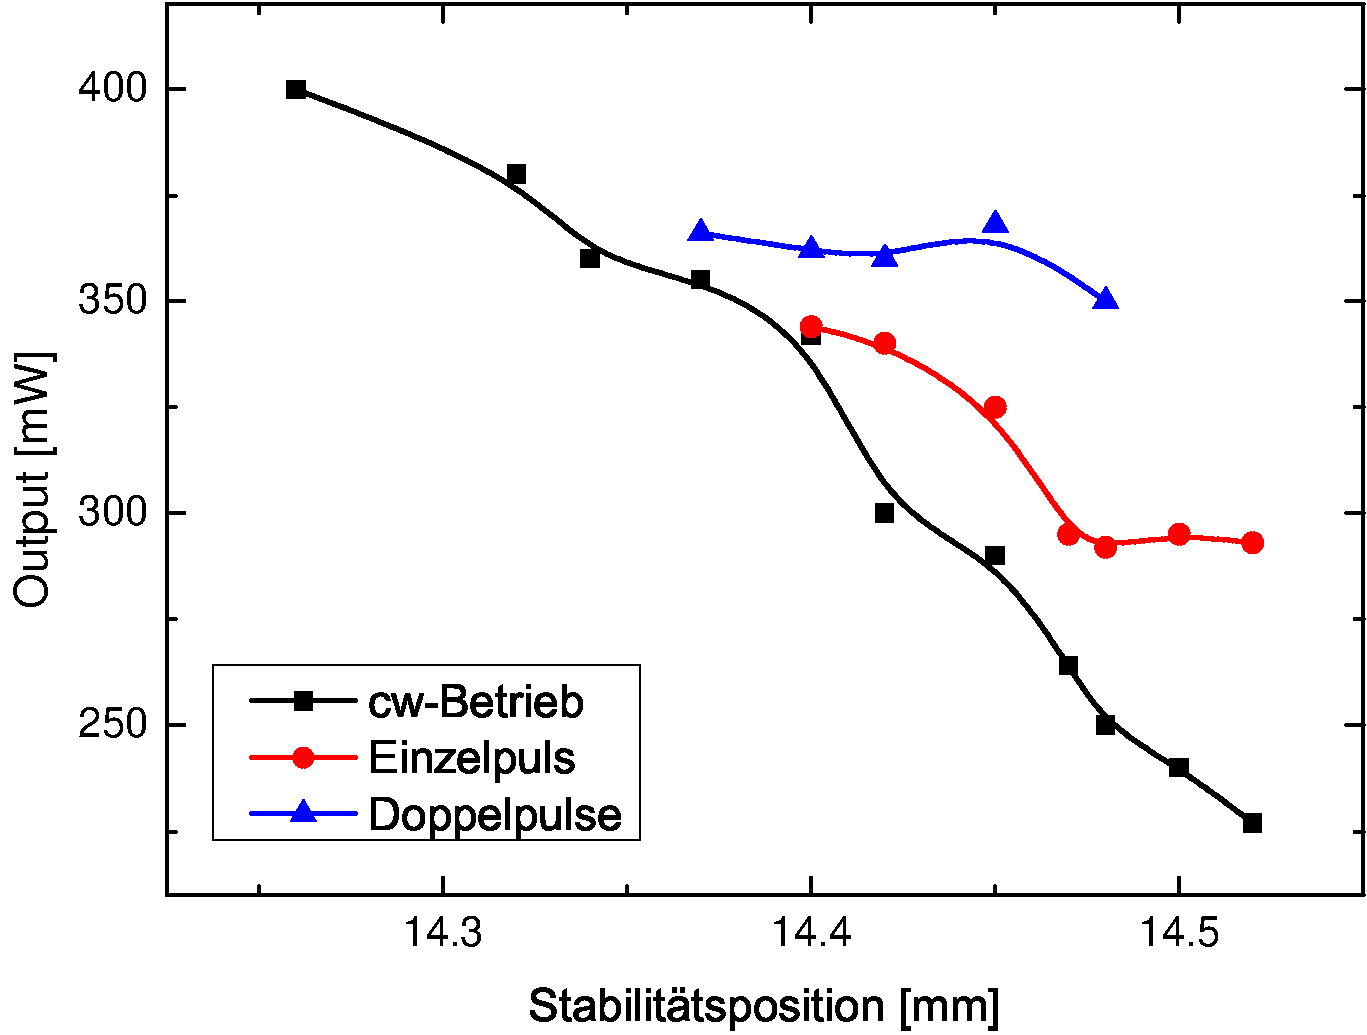
\includegraphics[width=0.7\textwidth]{figures/map2.pdf}
	\caption{Abhängigkeit der Ausgangsleistung (cw \& gemodelockt) von der Position des fokussierenden Spiegels (Stabilität) bei fester Kristallposition.}
	\label{fig:map2}
\end{figure}


\section{Darstellung der Messdaten}
Um durch eine langen Messung mit dem Oszilloskop die Entwicklung des Spektrums, etc. darstellen zu können, muss erst die Pulswiederholrate bestimmt werden.
Dies geschieht über eine Fouriertransformation des ganzen Signals.
Die Frequenz des höchsten Peaks entspricht der Wiederholrate, das Inverse davon also dem Pulsabstand $t_\text{rep}$ bzw. der optischen Cavity-Länge des Lasers.
Da sich diese zum Starten ändert, ist die bestimmte Wiederholrate nur für einen kurzen Ausschnitt der Messung korrekt.
Ist also $t_\text{rep}$ bestimmt, wird festgelegt, in wie viele äquidistante Punkte diese Zeit unterteilt werden soll.
Dies sollte so gewählt sein, dass die Abstände in etwa zugehörigen Samplingrate entspricht.
Dann werden die Messdaten an den neuen Zeitpunkten interpoliert und anschließend als Matrix dargestellt, trennt also jeden Roundtrip.
Die eine Achse entspricht den Roundtrips, die andere ist die Zeitachse pro Roundtrip.

Zuletzt muss noch die Änderung der Repetitionsrate bzw. die Abweichung vom richtigen Wert korrigiert werden.
Dies kann auf zwei Arten geschehen:
Ist der Anteil an der Messung, bei der der Laser gemodelockt ist, groß, wird ein Polynom durch die Peakpositionen des undispergierten, gemodelockten Signals gelegt, der Definitionsbereichs des Polynoms wird auf die gesamte Messung ausgedehnt und dann wird jeder Roundtrip so verschoben, dass diese Peakpositionen konstant sind.
Mit dem gleichen Polynom (nur mit einem anderen Offset) wird auch die dispergierte Messung verschoben.
Ist der Anteil an der Messung, bei der der Laser gemodelockt ist, jedoch kleiner, sodass ein großer Fehler gemacht wird, wenn das wie oben gefittete Polynom auch auf den nicht-gemodelockten Bereich ausgedehnt wird, muss sich einer anderen Methode bedient werden, um die Änderung der Rep.rate zu korrigieren.
Dies basiert auf der Korrelation zwischen zwei Roundtrips, immer davon ausgehend, dass sich zwischen zwei aufeinanderfolgenden Roundtrips kaum etwas ändert.
Man beginnt mit einem gemodelockten Spektrum und geht von diesem Spektrum zu früheren Roundtrips und bestimmt zu diesem die Korrelation.
Sollte der maximale Wert nicht bei der Verschiebung $\tau=0$ der beiden Signale zueinander sein, verschiebt man diesen Roundtrip um eben diesen Wert, sodass die Korrelation nun maximal bei $\tau=0$ ist.
Nun wird dieser Roundtrip (allerdings unverschoben) als neue Referenz genommen.
Das Spiel beginnt von vorne, es wird wieder die Korrelation zwischen diesem und vorigen Roundtrips gebildet, etc.
Allerdings wird die benötigte Verschiebung logischerweise aufsummiert.
Es hat sich als sinnvoll erwiesen, als Referenz nicht nur einen Roundtrip zu wählen, sondern die Mittlung über mehrere.
Das macht das Verfahren unsensibel gegenüber Rauschen in den Messdaten, die zu zu starken Verschiebungen führen.

\section{Doppelpulse Messreihe 1}
\subsection{Gebundene Pulse (hohe Pumpleistung)}
In diesem Zustand ändert sich der Abstand der Pulse nicht gravierend.
Es gibt jedoch ein oszillatorisches Verhalten der Phase und des Abstandes.
Für drei der in Abbildung \ref{fig:boundSpectro} gezeigten Messreihen ist dieses Verhalten in die \textit{Interaction Plane} eingezeichnet, also ein polarer Plot mit dem Abstand als Radius und der Phase als Winkel.
In Abbildung \ref{fig:interactionPlane} ist jedoch der Radius der um 80\,fs verringerte Abstand, damit Abstandsänderungen gut zu erkennen sind.
Zusätzlich sind Pfeile eingezeichnet, die anzeigen in welche Richtung die Orbits durchlaufen werden.
\begin{figure}[!htb]
   \centering
   \captionsetup[subfigure]{labelformat=empty}
   \captionsetup[subfloat]{farskip=-10pt,captionskip=0pt}
   \subfloat[\label{fig:rBF458}]
   {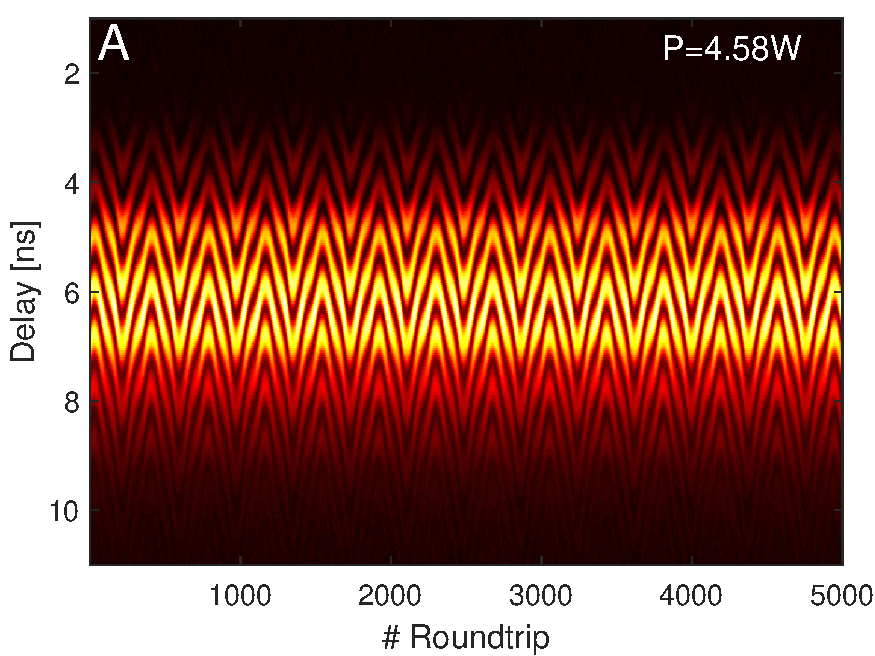
\includegraphics[width=0.49\textwidth]{figures/4ms_25GSA_400m_MLrun_runBounceFix_4,58W_Ch_PWnoCB111}}
   \hfill
   \subfloat[\label{fig:rBF463}]
   {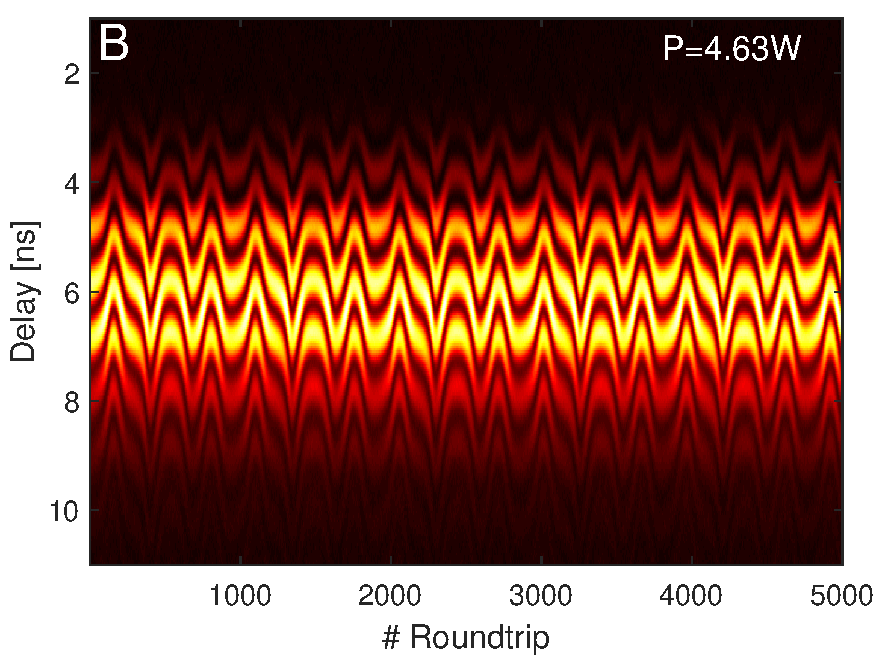
\includegraphics[width=0.49\textwidth]{figures/4ms_25GSA_400m_MLrun_runBounceFix_4,63W_Ch_PWnoCB111}}
   
   \subfloat[\label{fig:rBF464}]
   {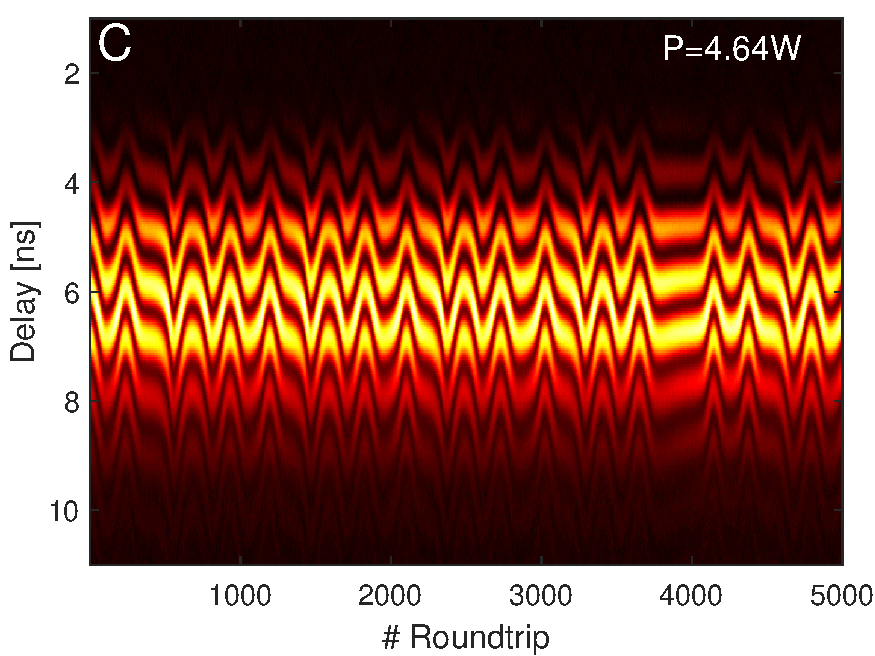
\includegraphics[width=0.49\textwidth]{figures/4ms_25GSA_400m_MLrun_runBounceFix_4,64W_Ch_PWnoCB111}}
   \hfill
   \subfloat[\label{fig:rBF468}]
   {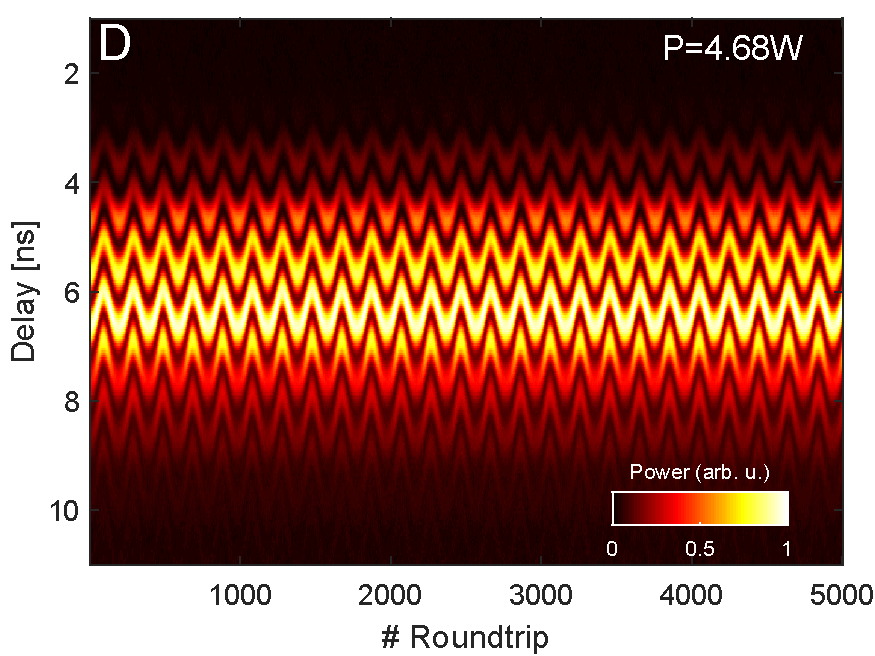
\includegraphics[width=0.49\textwidth]{figures/4ms_25GSA_400m_MLrun_runBounceFix_4,68W_Ch_PWwithCB111_0}}
   \caption{Bound Solitons: Spektren bei Änderung der Pumpleistung.}
   \label{fig:boundSpectro}
 \end{figure}
 
 \begin{figure}[!htb]
	\centering
	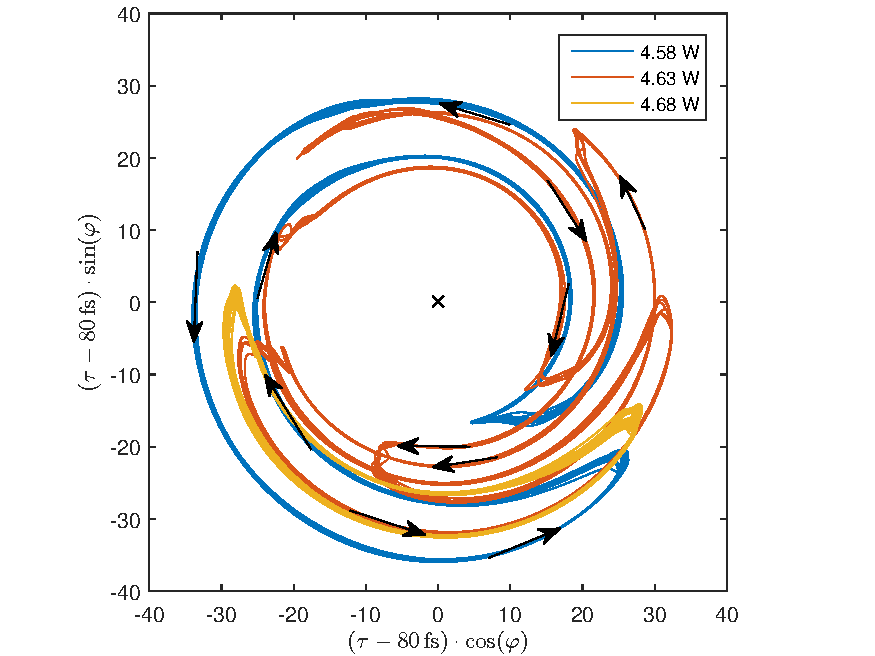
\includegraphics[width=0.8\textwidth]{figures/4ms_25GSA_400m_MLrun_runBounceFix_InteractionPlaneArrows2.pdf}
	\caption{Phasendynamik in der Interaction Plane.}
	\label{fig:interactionPlane}
\end{figure}

\subsection{Kollidierende Pulse (mittlere Pumpleistung)}
Dieser Zustand ist dadurch gekennzeichnet, dass es ständig zu Kollisionen zwischen den beiden Pulsen kommt, wie in Abbildung \ref{fig:rBF456} gut zu erkennen ist.
Diese entfernen sich danach schnell voneinander bevor der Abstand beider Pulse linear abnimmt und es schließlich zur erneuten Kollision kommt.
Erklären lässt sich dies damit, dass sich nach der Kollision ein schwacher Puls vor dem starken ausbildet, dieser aufgrund des Kerr-Effektes schneller durch die Cavity läuft und somit der Abstand beider größer wird.
Dann kommt es jedoch zu einem Erstarken des vorderen Pulses und zu einer Schwächung des hinteren, weil der hintere nur die schon vom vorderen reduzierte Besetzungsinversion sieht und so weniger Verstärkung bekommt.
Es stellt sich ein fixes Intensitätsverhältnis und somit auch eine konstante Relativgeschwindigkeit ein, sodass sich beide mit dieser annähern bis es zur nächsten Kollision kommt.
Somit lässt sich auch erklären, warum die Kollisionszeit $T_\text{interColl.}$, also die Zeit zwischen zwei Kollisionen linear mit der maximalen Entfernung $\tau_\text{max}$ zusammenhängt (Abb. \ref{fig:bounceDistTime}).

\begin{figure}[!htb]
   \centering   
   \subfloat[Ausschnitt der Autokorrelation\label{fig:rBF456}]
   {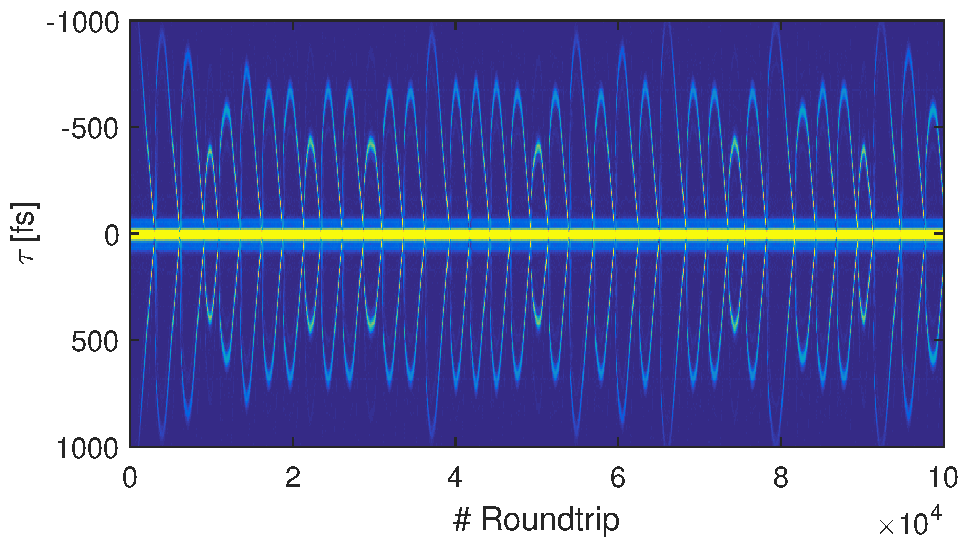
\includegraphics[width=0.58\textwidth]{figures/4ms_25GSA_400m_MLrun_runBounceFix_4,56W_Ch1_150000_250000_autocorr_stretch}}
   \hfill
   \subfloat[Histogramm des maximalen Pulsabstandes $\tau_\text{max}$ pro Bounce\label{fig:rBF456histo}]
   {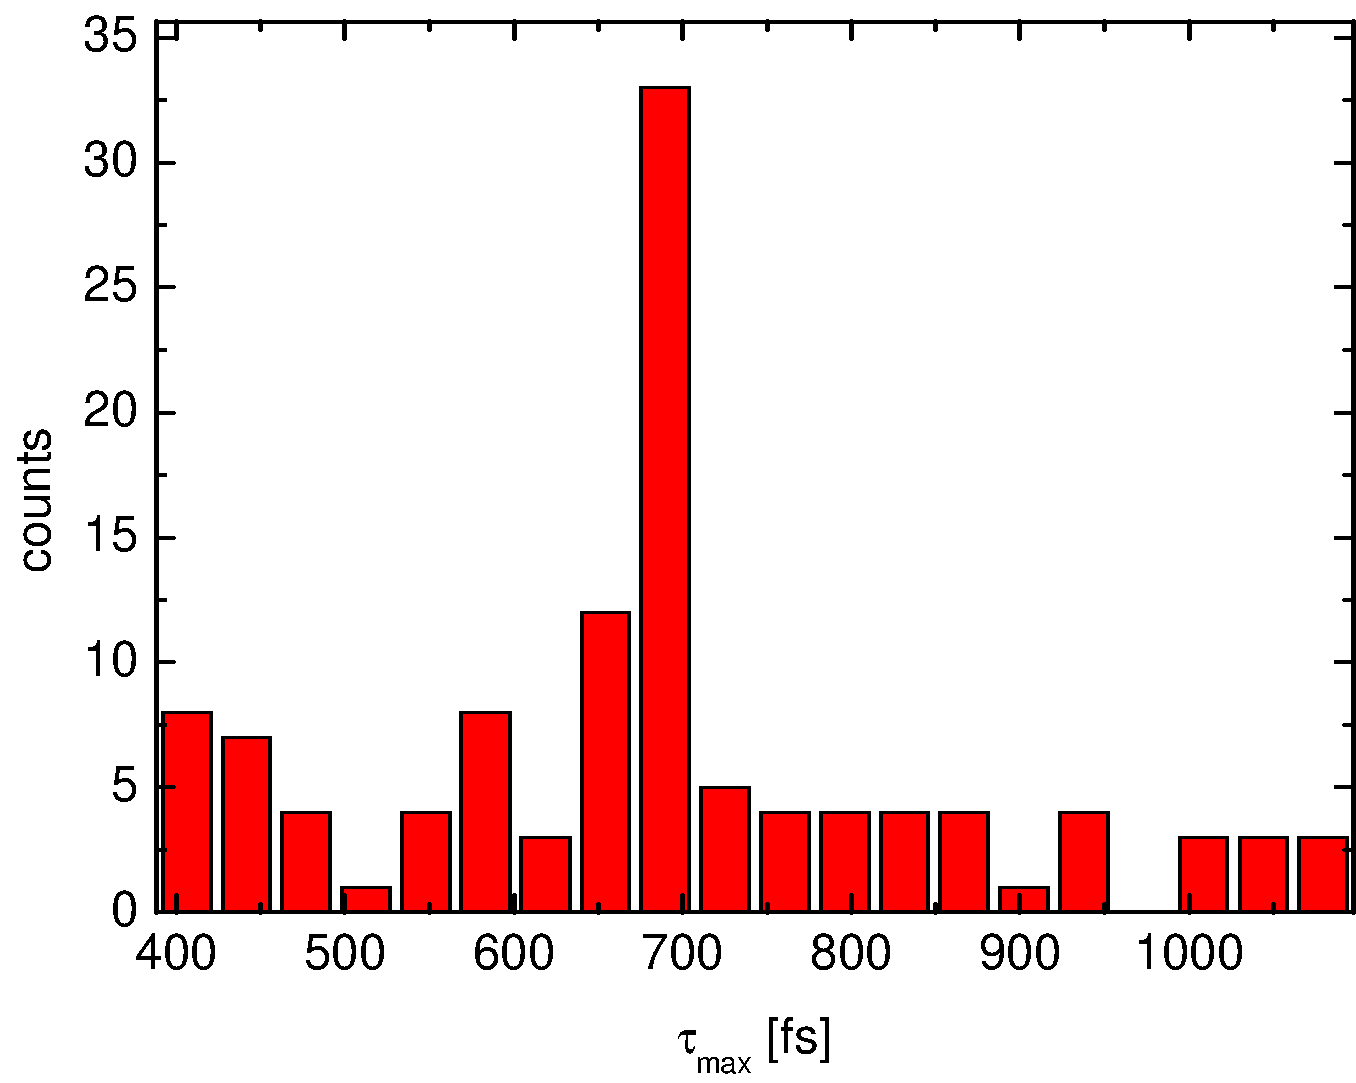
\includegraphics[width=0.4\textwidth]{figures/bounce456histo}}
   \caption{Bouncing-Mode bei einer Pumpleistung von $4.56\,$W.}
   \label{fig:bouncing456}
 \end{figure}

Wenn die Pumpleistung auf 4.57\,W erhöht wird, zeigt sich noch ein weiterer Interaktionsmechanismus: Die beiden Pulse stoßen sich voneinander ab, bevor sie überhaupt kollidieren.

\begin{figure}[!htb]
   \centering
   \subfloat[Überblick.\label{fig:rBF457_autocorr}]
   {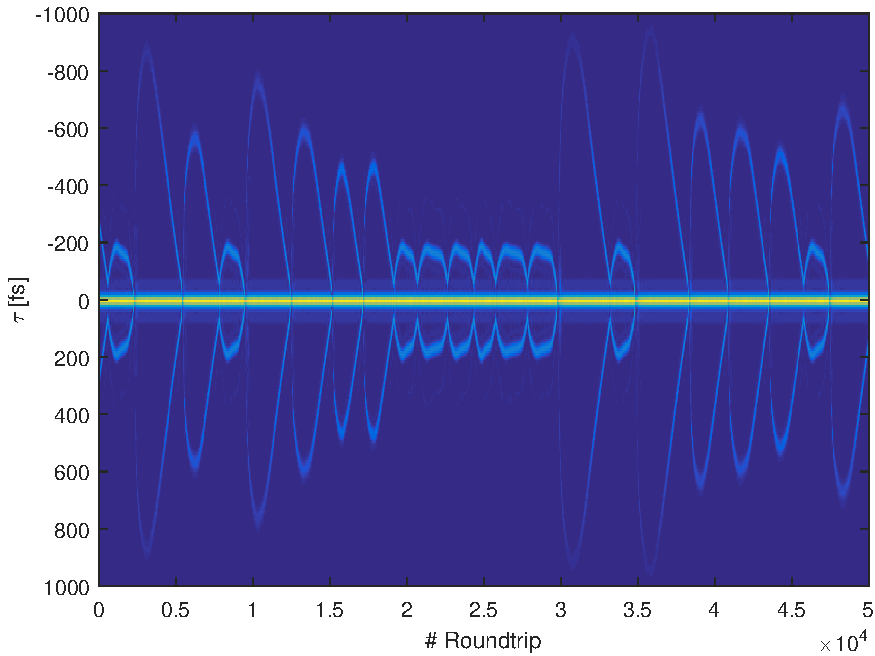
\includegraphics[width=0.49\textwidth]{figures/4ms_25GSA_400m_MLrun_runBounceFix_4,57W_Ch1_120000_170000_autocorr}}
   \hfill
   \subfloat[Zoom.\label{fig:rBF457_autocorr_zoom}]
   {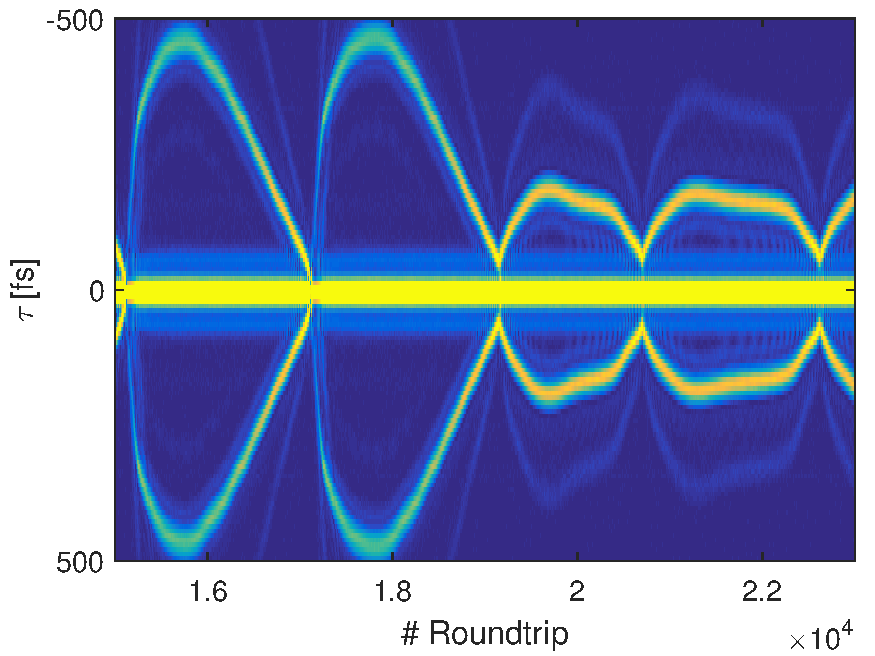
\includegraphics[width=0.49\textwidth]{figures/4ms_25GSA_400m_MLrun_runBounceFix_4,57W_Ch1_135000_143000_autocorr}}
   
   \subfloat[Kollision, spektrale Ansicht.\label{fig:rBF457_coll_spec}]
   {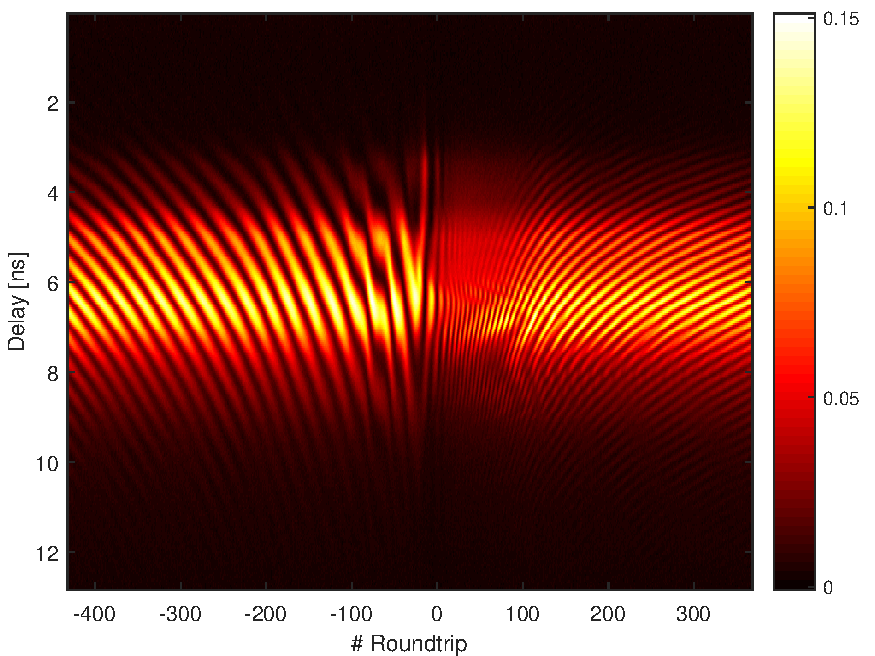
\includegraphics[width=0.49\textwidth]{figures/4ms_25GSA_400m_MLrun_runBounceFix_4,57W_Ch1_136700_137500_spectrum}}
   \hfill
   \subfloat[Kollision, Autokorellation.\label{fig:rBF457_coll_autocorr}]
   {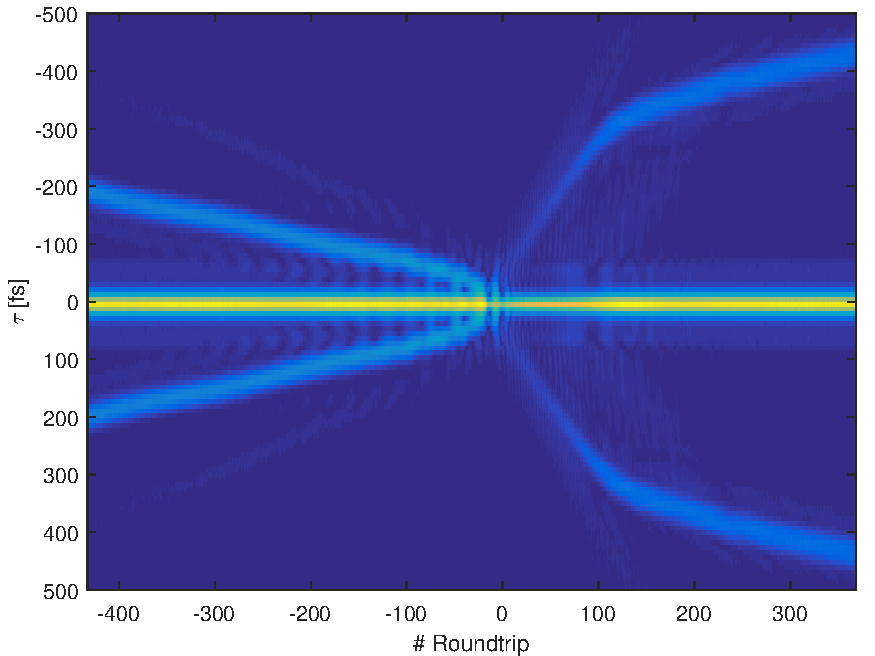
\includegraphics[width=0.49\textwidth]{figures/4ms_25GSA_400m_MLrun_runBounceFix_4,57W_Ch1_136700_137500_autocorr}}
   
   \subfloat[Abstoßung, spektrale Ansicht.\label{fig:rBF457_repel_spec}]
   {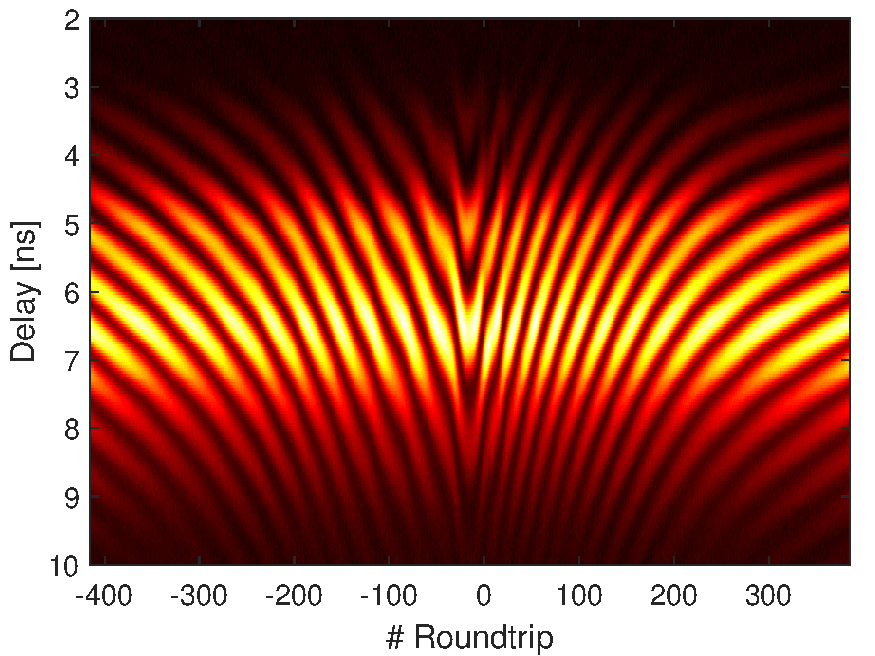
\includegraphics[width=0.49\textwidth]{figures/4ms_25GSA_400m_MLrun_runBounceFix_4,57W_Ch1_140300_141100_spectrum}}
   \hfill
   \subfloat[Abstoßung, Autokorrelation.\label{fig:rBF457_repel_autocorr}]
   {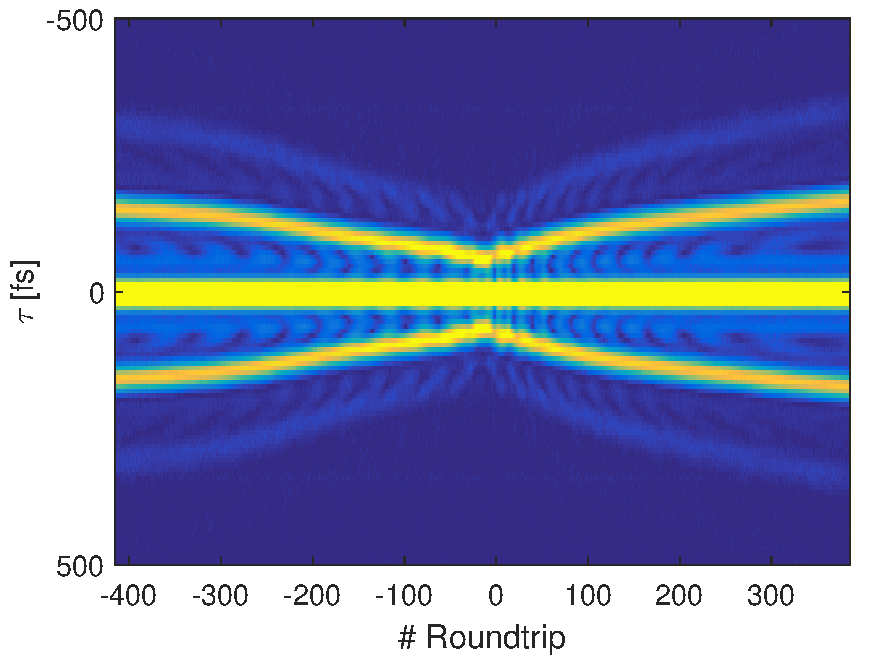
\includegraphics[width=0.49\textwidth]{figures/4ms_25GSA_400m_MLrun_runBounceFix_4,57W_Ch1_140300_141100_autocorr}}
   \caption{$P_\text{Pump}=4.57\,$W: Unterschied zwischen Kollision und Abstoßung der beiden Pulse.}
   \label{fig:rbf457}
 \end{figure}

\begin{figure}[!htb]
	\centering
	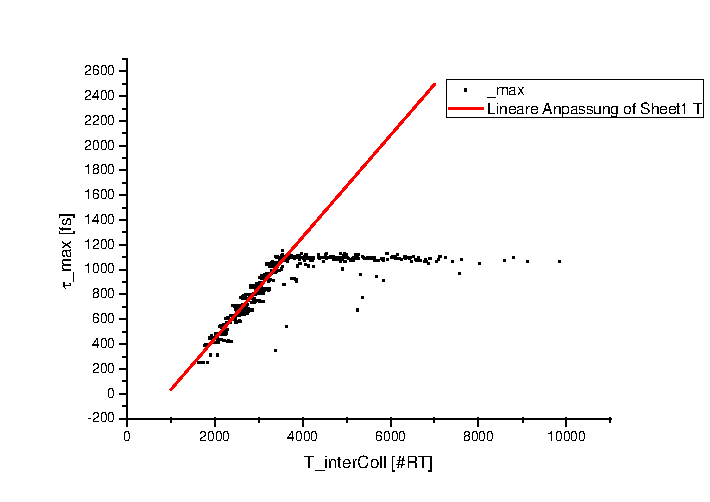
\includegraphics[width=0.8\textwidth]{figures/bounceDistTime}
	\caption{Maximaler Pulsabstand $\tau_\text{max}$ versus Zeit zwischen zwischen zwei Kollisionen $T_\text{interColl.}$. Das bestimmte $\tau_\text{max}$ ist begrenzt durch die maximale Modulationsfrequenz des Spektrums.}
	\label{fig:bounceDistTime}
\end{figure}

\subsection{Durchlaufende Pulse (niedrige Pumpleistung)}
In diesem Zustand ist die Pumpleistung so gering, dass zwar zwei Pulse durch den Laser laufen, diese aber einen großen Intensitätsunterschied haben, so dass sie unterschiedliche optische Weglängen haben und sich so auf einer Skala von 100\,ms gegeneinander verschieben.
In Abb. \ref{fig:rBF441} ist eine \textit{FastFrame}-Aufnahme dieses Betriebs zu sehen.
Dabei wird auf den stärkeren Puls getriggert und im Gegensatz zu den anderen Aufnahmen ist dies keine kontinuierliche Messung, bei der zu jedem Roundtrip das Spektrum und zeitliches Signal aufgenommen wird.
Hier werden sehr viele Pulse übersprungen, damit eine solch lange Zeit mit so einer gleich hohen Samplingrate aufgenommen werden kann.

Genauer hinschauend erkennt man, dass die Relativgeschwindigkeit zwischen beiden Pulsen nur annähernd konstant ist.
Dies lässt sich auch in der Peak-Spannung des undispergierten Signals erkennen, welche proportional zur Pulsenergie ist.
So wird der schwache Puls die meiste Zeit schwächer während der starke stärker wird.
Dies führt zu einer Zunahme der Relativgeschwindigkeit.
Es gibt jedoch zwei Zeitpunkte zwischen zwei aufeinanderfolgenden Kollisionen, bei denen sich dieses Verhalten genau umgekehrt: Es findet ein Energietransfer vom stärkeren zum schwächeren Puls statt und die Relativgeschwindigkeit nimmt ab.
Dies lässt sich damit erklären, dass die beiden Pulse sich gerade dann im Laserkristall begegnen und so der schwächere Puls vom Kerr-Effekt durch den stärkeren profitiert.

\begin{figure}[!htb]
   \centering   
   \subfloat[\textit{FastFrame}-Aufnahme\label{fig:rBF441}]
   {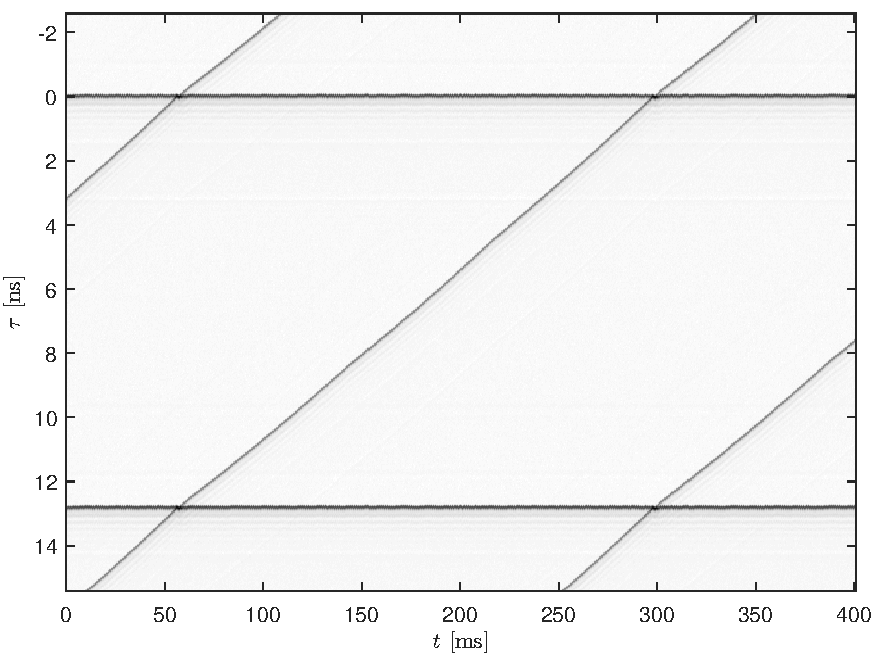
\includegraphics[width=0.49\textwidth]{figures/400ms_5musHold_25GSA_400m_MLrun_runBounceFix_4,41W_Ch2}}
   \hfill
   \subfloat[\label{fig:rBF441peakTau}]
   {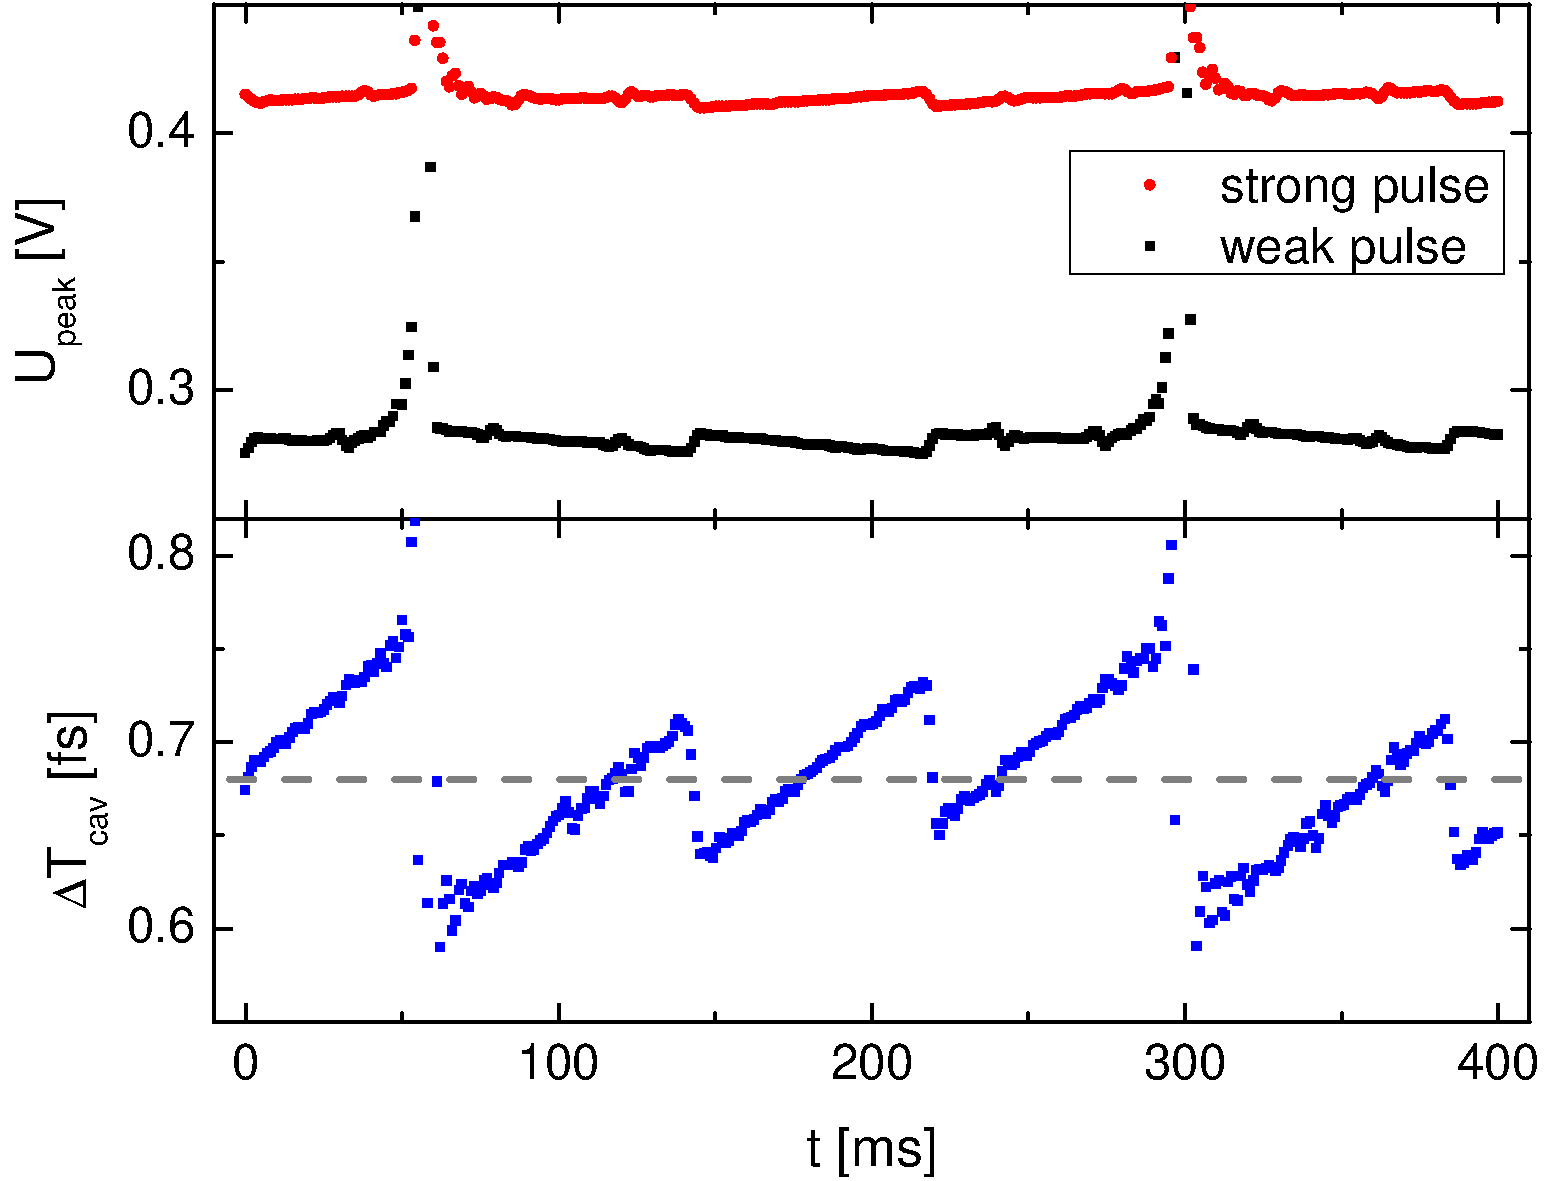
\includegraphics[width=0.49\textwidth]{figures/runningPeakTau}}
   \caption{Zwei unterschiedlich starke Pulse im Laser, die aufgrund des Kerr-Effekts verschiedene optische Weglängen sehen und sich so gegeneinander verschieben.}
   \label{fig:running441}
 \end{figure}


\section{Doppelpulse Messreihe 2}
\subsection{Stufenweise Phasenentwicklung gebundener Doppelpulse}
Hier beginnt die Messreihe mit Doppelpulsen, deren Phase und relativer Abstand fix sind.
Der Abstand liegt etwa bei 170 \,fs.
Dann wird die Pumpleistung verringert.
Dabei wird beobachtet, dass der Abstand der beiden Pulse immer noch sehr konstant ist, während die Phase jedoch beginnt, in Schüben/Sprüngen durchzulaufen.
Dies deutet auf einen Intensitätsunterschied zwischen beiden Pulsen hin.
Die Phase läuft jedoch nicht linear durch, sondern bildet Stufen.
Nach XXX ist die Phase bei $\varphi=\pm\pi/2$ gelockt.
Vermutlich kann in der Umgebung von diesem Wert die fehlende Energie noch durch Senkung beider Pulsamplituden aufgefangen werden, was zu einer annähernd konstanten Phase führt, wohingegen diese ab einer bestimmten Abweichung von $\pi/2$ sich in sehr kurzer Zeit um fast $2\pi$ ändert.
Dies könnte bedeuten, dass dann der vordere sehr schnell stärker und der hintere schwächer wird, bis die Phase erneut etwas kleiner als $\pi/2$ ist und beide Pulse ihre Amplituden angleichen.
Verringert sich die Pumpleistung weiter, geschieht dieser Prozess schneller, bis die Phase annähernd linear durchläuft.
\begin{figure}[!htb]
   \centering
   \captionsetup[subfigure]{labelformat=empty}
   \captionsetup[subfloat]{farskip=-10pt,captionskip=0pt}
   \subfloat[]{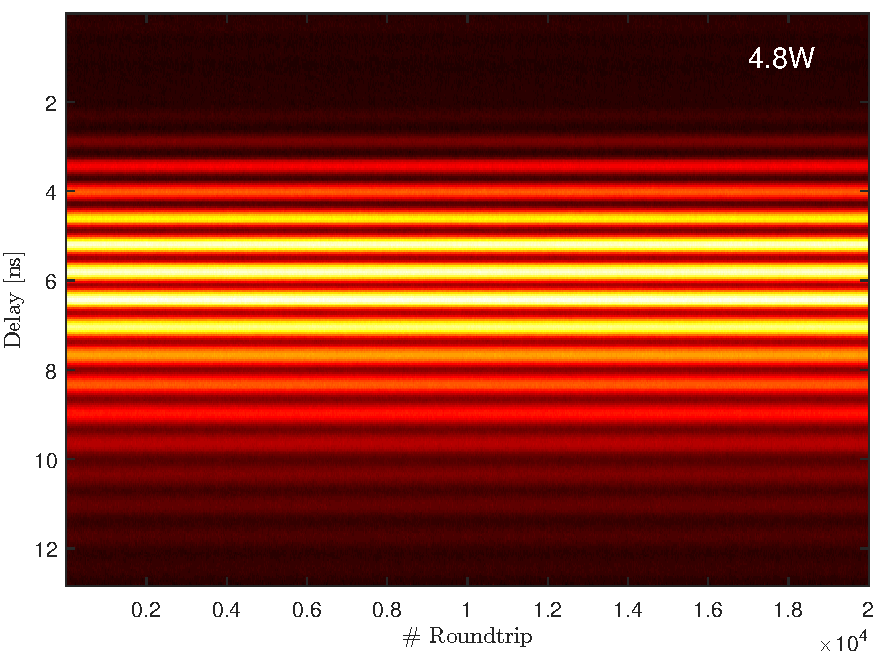
\includegraphics[width=0.49\textwidth]{figures/4ms_25GSA_400m_MLrun_Doppel4,8W_2_Ch_PWnoCB}}
   \hfill
   \subfloat[]
   {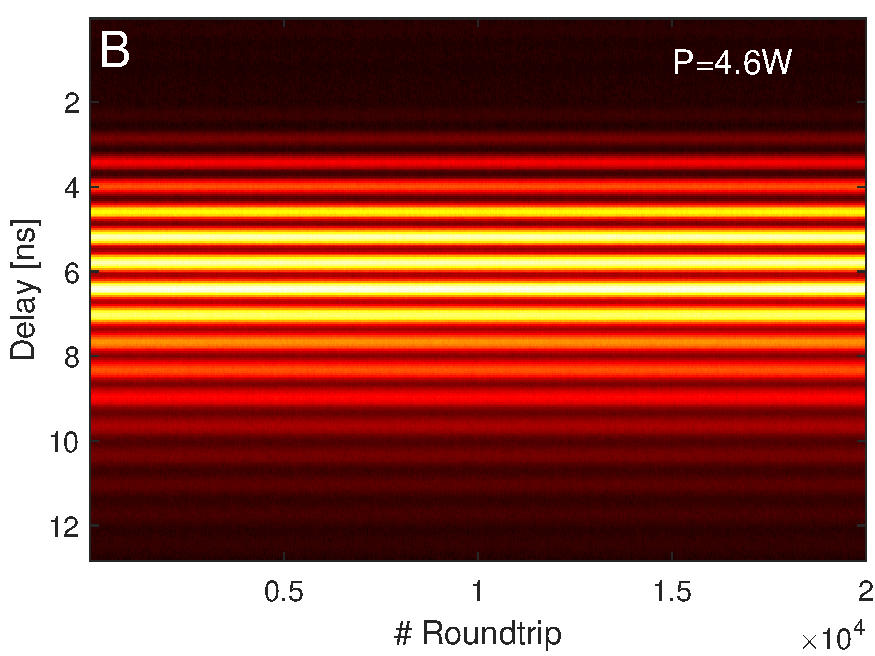
\includegraphics[width=0.49\textwidth]{figures/4ms_25GSA_400m_MLrun_Doppel4,6W_Ch_PWnoCB}}
   %\hfill
   
   \subfloat[]
   {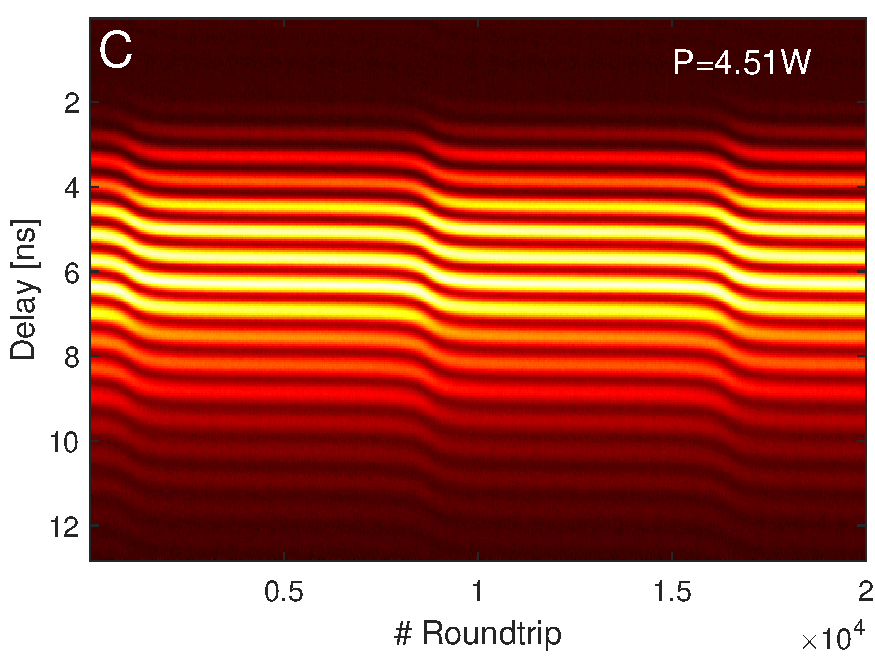
\includegraphics[width=0.49\textwidth]{figures/4ms_25GSA_400m_MLrun_Doppel4,51W_Ch_PWnoCB}}
   \hfill
   \subfloat[]
   {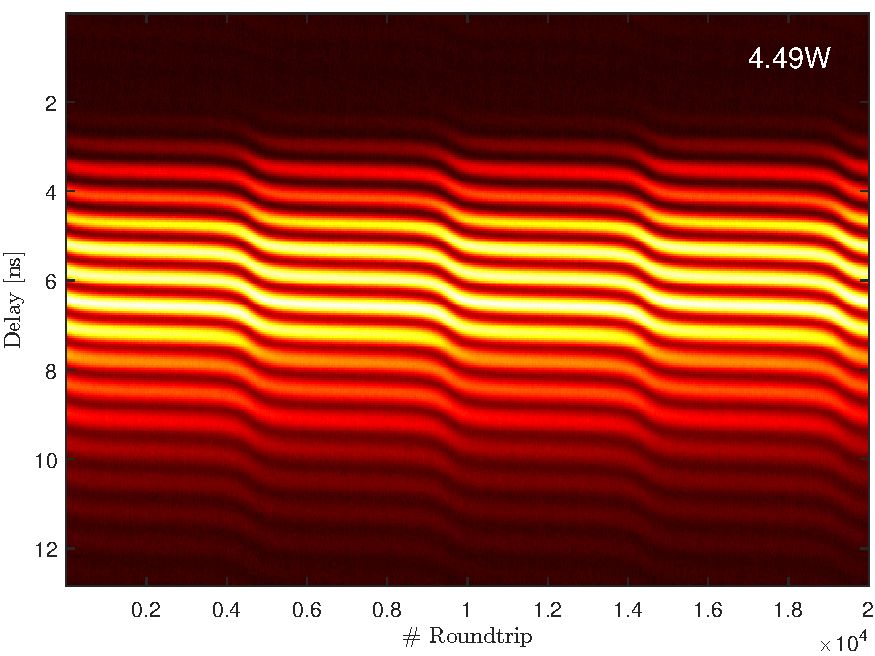
\includegraphics[width=0.49\textwidth]{figures/4ms_25GSA_400m_MLrun_Doppel4,49W_Ch_PWnoCB}}
   %\hfill
   
   \subfloat[]
   {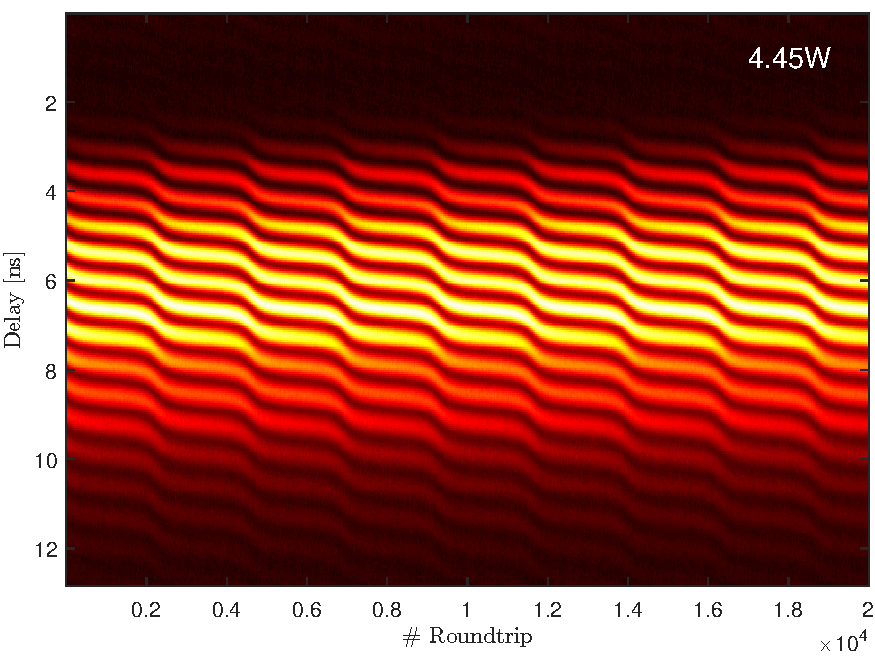
\includegraphics[width=0.49\textwidth]{figures/4ms_25GSA_400m_MLrun_Doppel4,45W_2_Ch_PWnoCB}}
   \hfill
   \subfloat[]
   {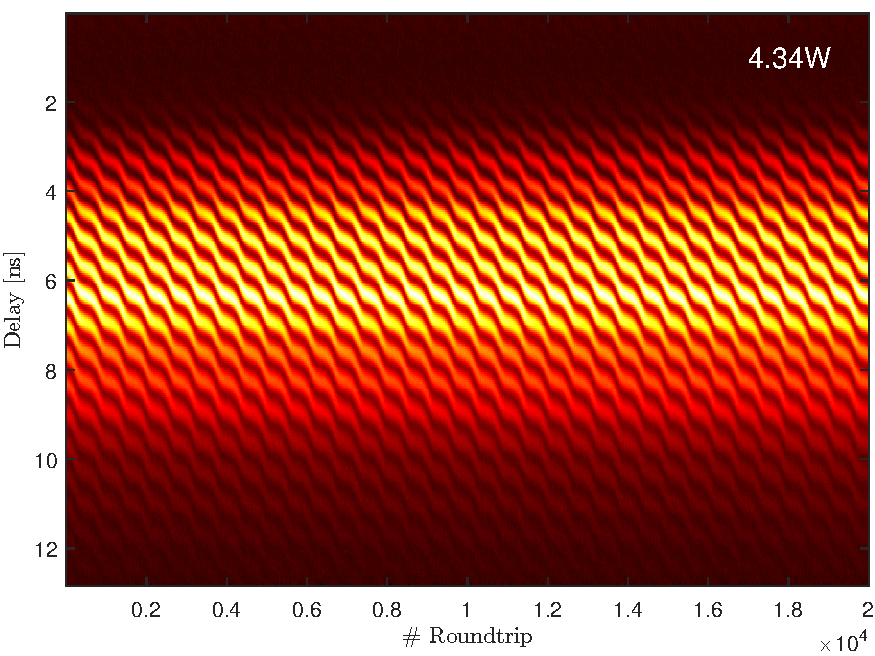
\includegraphics[width=0.49\textwidth]{figures/4ms_25GSA_400m_MLrun_Doppel4,34W_Ch_PWnoCB}}
   %\hfill
   
   \subfloat[]
   {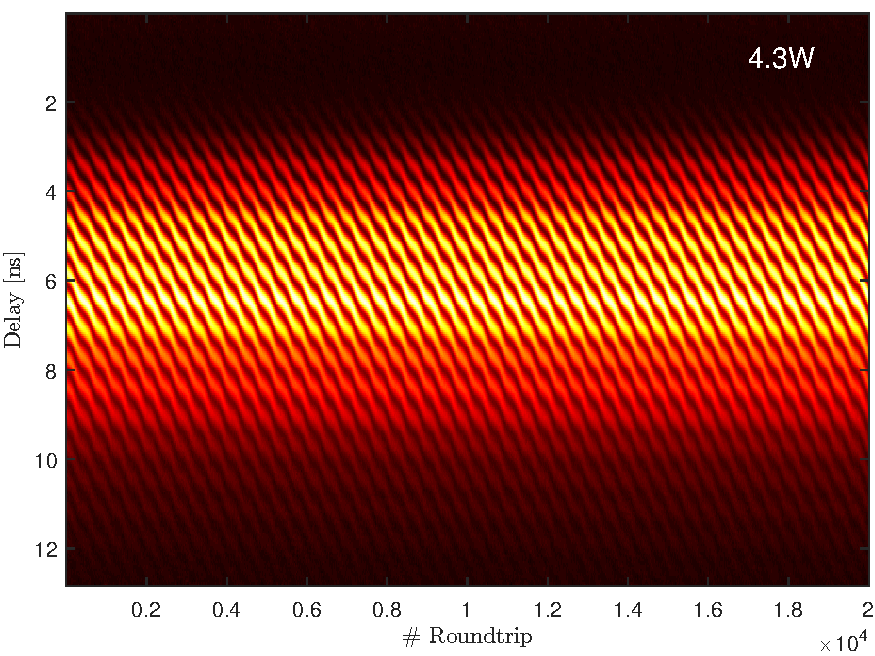
\includegraphics[width=0.49\textwidth]{figures/4ms_25GSA_400m_MLrun_Doppel4,3W_Ch_PWnoCB}}
   \hfill
   \subfloat[]
   {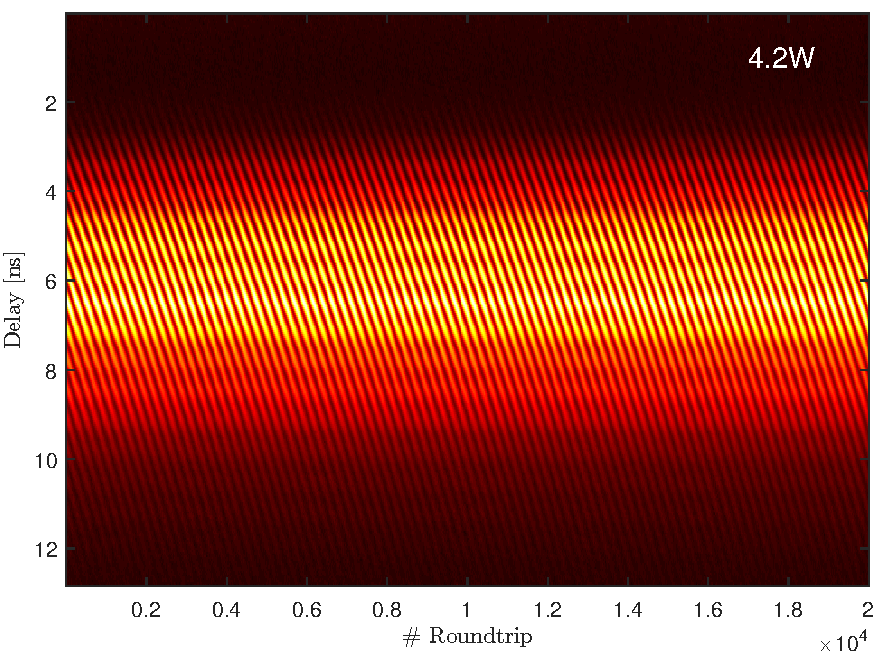
\includegraphics[width=0.49\textwidth]{figures/4ms_25GSA_400m_MLrun_Doppel4,2W_Ch_PWnoCB}}
   \caption{Verringerung der Pumpleistung: Von einer festen Phase über Stufen zu einer annähernd linear durchlaufenden Phase.}
   \label{fig:165014steps}
 \end{figure}
 
\begin{figure}
	\centering
	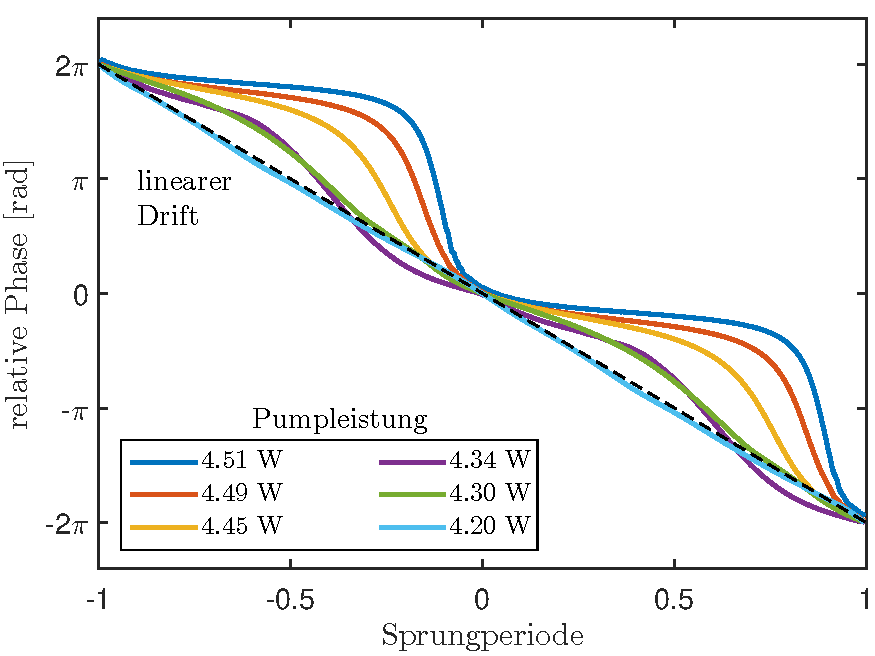
\includegraphics[width=0.7\textwidth]{figures/steps_relativ2.pdf}
	\caption{Verringerung der Pumpleistung: Von einer festen Phase über Stufen zu einer annähernd linear durchlaufenden Phase.}
   \label{fig:165014steps2}
\end{figure}

\begin{figure}[!htb]
   \centering   
   \subfloat[benötigte Zeit\label{fig:jumpRT}]
   {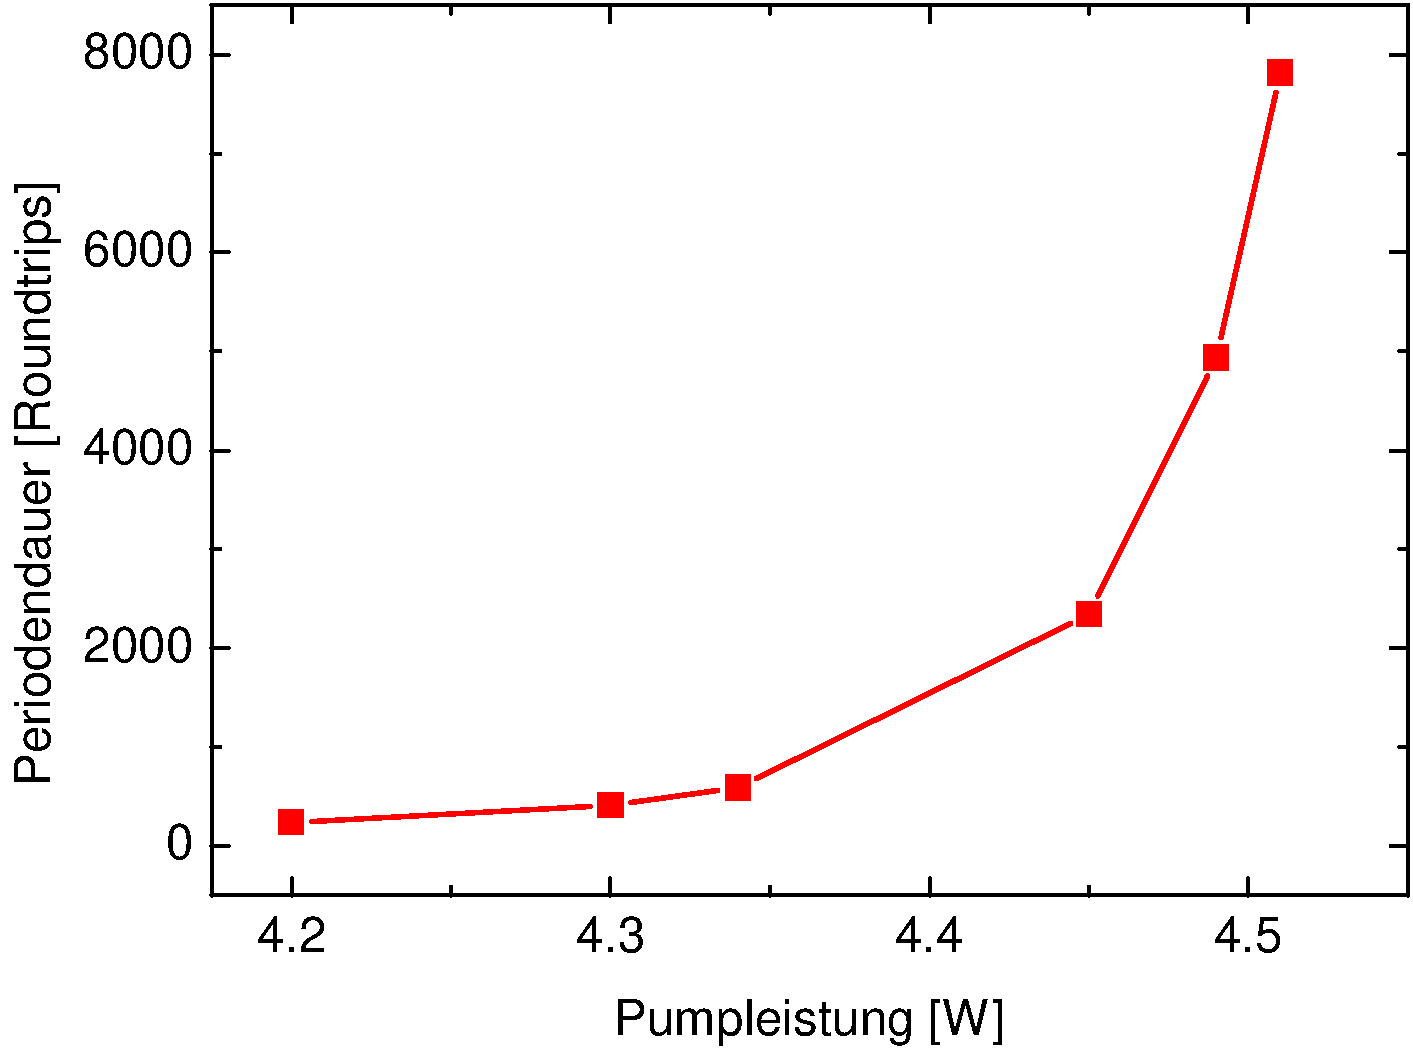
\includegraphics[width=0.49\textwidth]{figures/jumpRT}}
   \hfill
   \subfloat[\label{fig:steps2}]
   {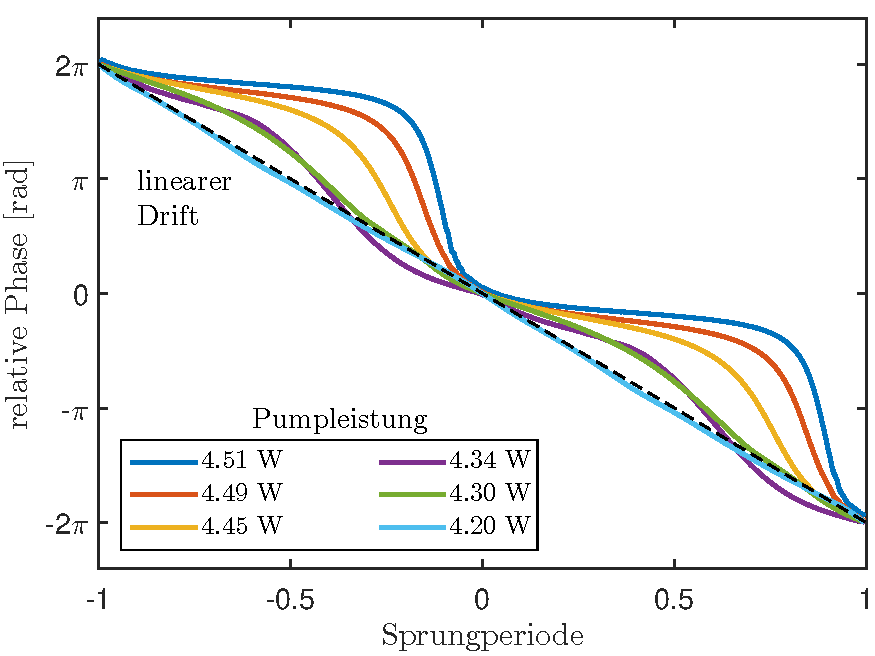
\includegraphics[width=0.49\textwidth]{figures/steps_relativ2}}
   \caption{Verringerung der Pumpleistung: Von einer festen Phase über Stufen zu einer annähernd linear durchlaufenden Phase.}
   \label{fig:160514steps2}
 \end{figure}
 
% \begin{figure}[!htb]
%   \centering
%   \captionsetup[subfigure]{labelformat=empty}
%   \captionsetup[subfloat]{farskip=-10pt,captionskip=0pt}
%   \subfloat[]
%   {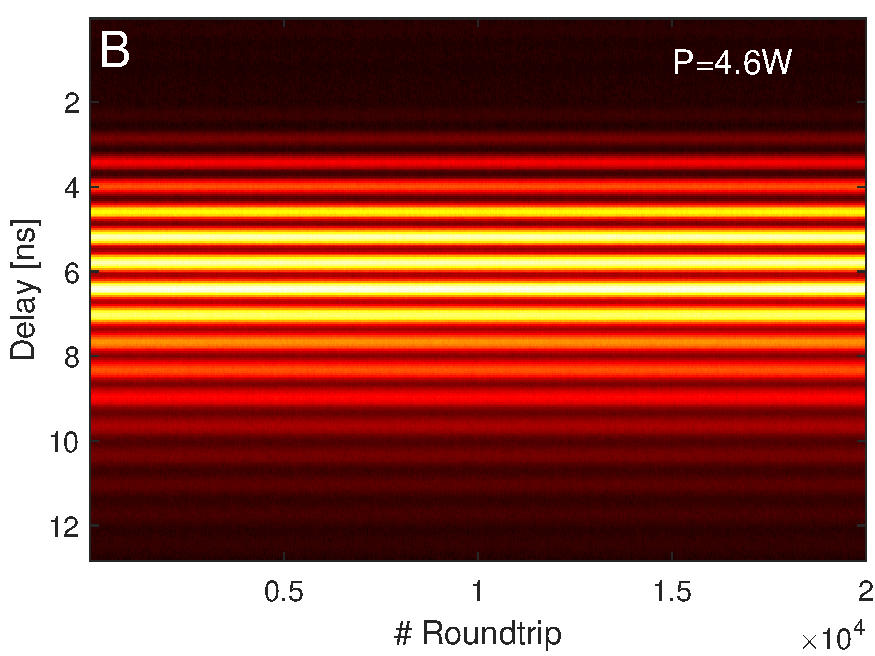
\includegraphics[width=0.49\textwidth]{figures/4ms_25GSA_400m_MLrun_Doppel4,6W_Ch_PWnoCB}}
%   \hfill
%   \subfloat[]
%   {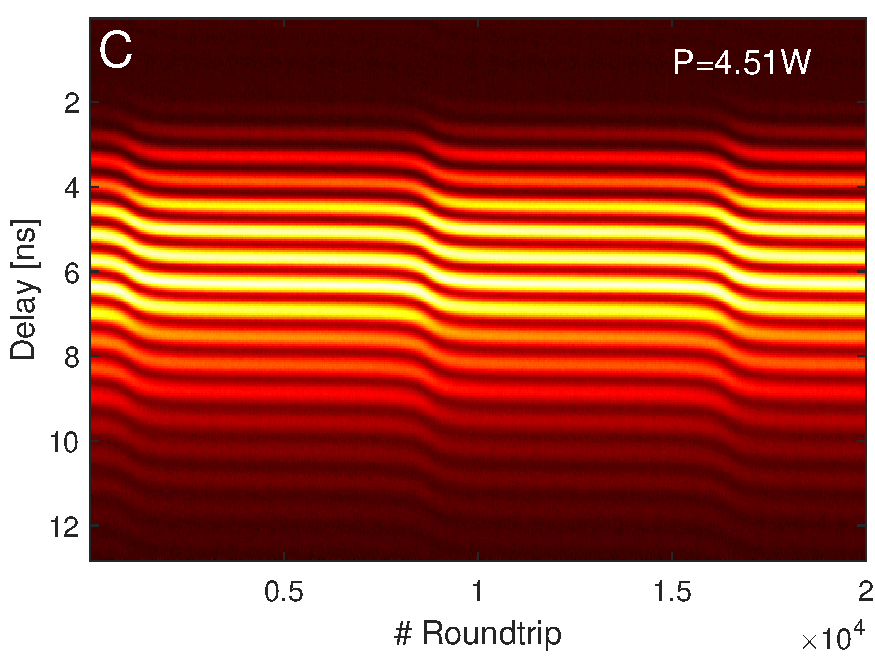
\includegraphics[width=0.49\textwidth]{figures/4ms_25GSA_400m_MLrun_Doppel4,51W_Ch_PWnoCB}}
%   
%   \subfloat[]
%   {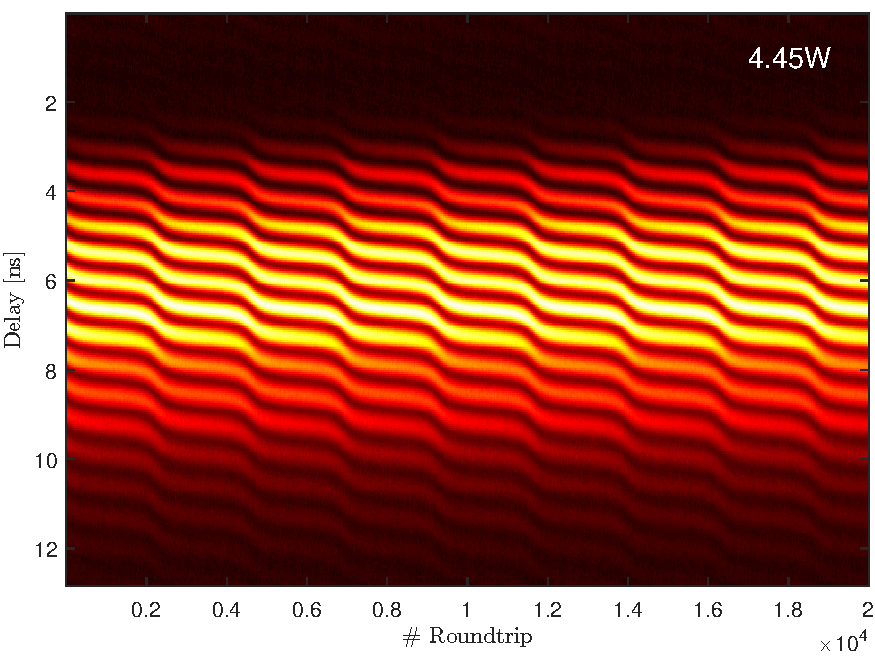
\includegraphics[width=0.49\textwidth]{figures/4ms_25GSA_400m_MLrun_Doppel4,45W_2_Ch_PWnoCB}}
%   \hfill
%   \subfloat[]
%   {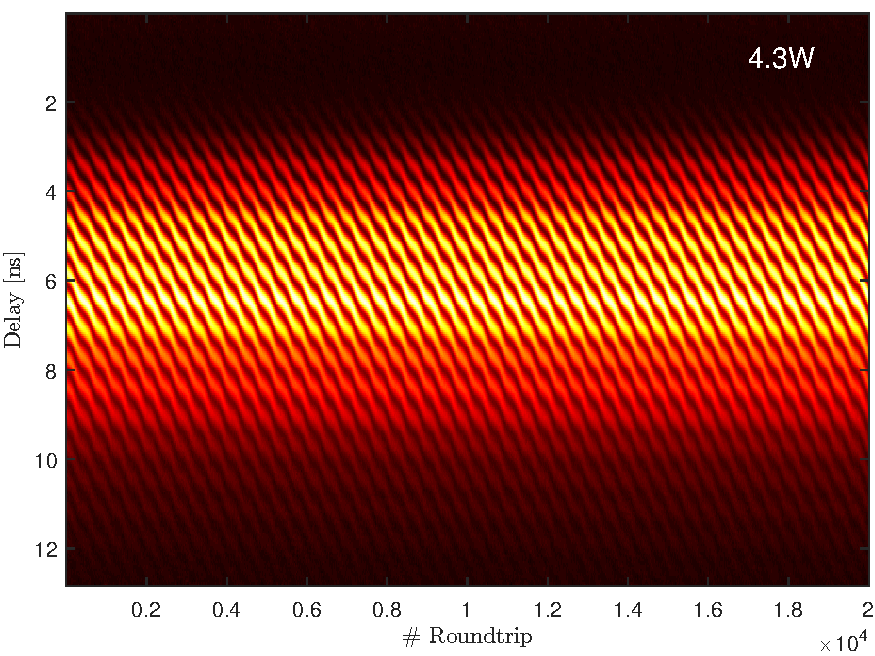
\includegraphics[width=0.49\textwidth]{figures/4ms_25GSA_400m_MLrun_Doppel4,3W_Ch_PWnoCB}}
%   \caption{Beschriftung allgemein}
%   \label{fig:label-gesamt}
% \end{figure}

\subsection{Dreifach-Pulse}

\section{Weiteres}

\chapter{Diskussion}
\section{Colliding Pulse Modelocking}
\label{sec:cpml}
Während der Messungen konnte das sogennante \textit{Colliding Pulse Modelocking} beobachtet werden.
Dabei laufen zwei Pulse im Laser umher, die sich im Laserkristall treffen und so den Kerr-Effekt beider Pulse sehen, sodass beide eine höhere Verstärkung erfahren.
Dieser Zustand ist sehr stabil und wurde zuerst von \cite{lai_multiple_1997} in einem Ti:Sa-Laser beschrieben.
Interessant ist nun der Prozess bevor dieser stabile Zustand erreicht wird.
Typischerweise modelockt eine Fluktuation, während die anderen Fluktuationen aber nicht völlig aussterben.
Eine weitere Fluktuation wächst nun an, sodass auch diese modelockt.
Daraufhin bewegen sich die beiden Pulse relativ zueinander, da sie nicht gleich stark sind und aufgrund des Kerr-Effektes unterschiedliche optische Weglängen im Laser haben.
Dies geschieht auf einer relativ langen Zeitskala (Größenordnung $~100\,$ms), ist also mit einer normalen Messung (nur 4\,ms) nicht aufzunehmen.
Dazu müsste in den \textit{FastFrame}-Mode gewechselt werden, in dem aber dann nicht jeder Puls aufgenommen werden kann.
Außerdem ist bei solch großen Abständen zwischen den Pulsen das undispergierte Signal das wichtigere.
Die Genauigkeit liegt dort aber nur bei ca. $10\,$ps.

Interessant zu beobachten wäre nun, wie der schwächere Puls das Wandern beendet.
Gleichen sich beide Pulse nur in ihrer Intensität an, dass sie beide genau dann gleich stark sind, wenn sie den perfekten Abstand zueinander haben?
Oder ist eine abklingende Schwingung um diesen zu beobachten?
Wie stabil ist dieser Abstand überhaupt, gibt es auch später noch Oszillationen?

Um all diese Fragen zu beantworten, könnte man den Strahl aufspalten und den einen Teil so verzögern, dass der erste Puls in diesem Arm zeitgleich mit dem zweiten Puls im kürzeren Abschnitt überlappt.
Nun ist die Abstandsinformation auch wieder im Spektrum einkodiert und der Abstand zwischen beiden Pulsen kann genau gemessen werden.

\section{Woher stammen die Doppelpulse?}
Splitting?
Modelockt eine andere Fluktuation?


\chapter{Zusammenfassung}
Laser ist komplex, Messmethode ist verdammt cool!

\appendix
\chapter{Femtolasers Rainbow CEP HP}
\begin{figure}[!htb]
	\centering
	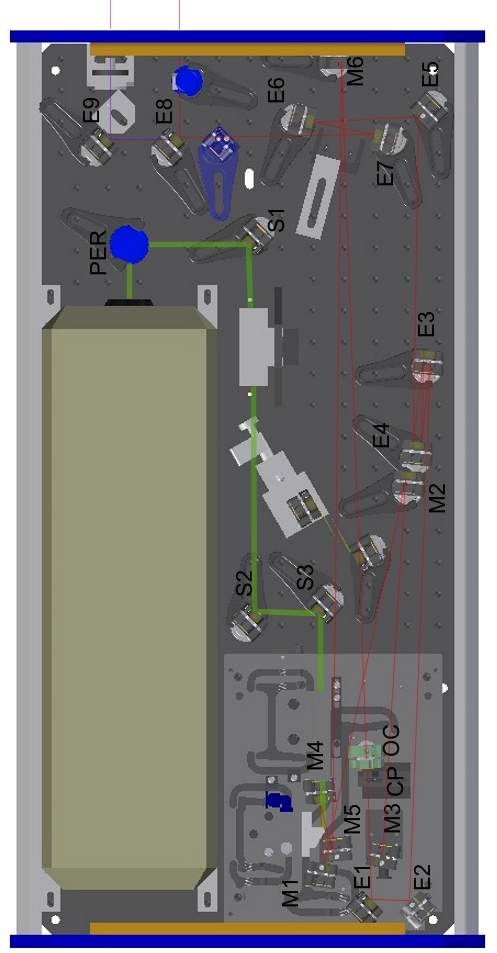
\includegraphics[width=0.6\textwidth]{figures/RainbowSetupManual.png}
\end{figure}
\chapter{Matlab-Code}
\section{Darstellung der Messdaten}

\section{Simulation}
\lstinputlisting[style=Matlab-editor]{SimulationRBcomment.m}

\cleardoublepage
%% Bibliographie. Das Argument muss der Name der BIBTeX-Datenbank stehen.
%% Ein Beispiel fuer eine solche Datenbank finden Sie in bthesis_datenbank.bib
\bibliography{test} 

\chapter*{Danksagung}
Ein besonderes Dankeschön geht an Dr. Christoph Bollig von \textit{Abacus Laser}, der das nötige Equipment und Know-How hatte, um die für das Experiment so wichtige dispersive Faser wieder zu spleißen, nachdem sie gerissen ist.
So konnte ich ohne lange Unterbrechung wieder weiter messen.

Außerdem bedanke ich mich bei der Elekronik-Werkstatt sowie der feinmechanischen Werkstatt des 4.Physikalischen Instituts für ihre kompetente und schnelle Unterstützung.

%% Dieser Befehl MUSS am Ende stehen und erzeugt die Erklaerung ueber die
%% benutzten Mittel
\Declaration
\end{document}
